\documentclass[12pt,letterpaper]{article}
\usepackage[utf8]{inputenc}
\usepackage[T1]{fontenc}
\usepackage[spanish,es-tabla]{babel}
\usepackage{times}
\usepackage[margin=2.54cm]{geometry}
\usepackage{setspace}
\usepackage{graphicx}
\usepackage{booktabs}
\usepackage{caption}
\usepackage{float}
\usepackage{fancyhdr}
\usepackage{xcolor}
\usepackage{enumitem}
\usepackage[hidelinks]{hyperref}
\usepackage{xurl}
\usepackage{titlesec}
\usepackage{amsmath}
\usepackage{tabularx}

\definecolor{naranja}{RGB}{232,89,12}
\definecolor{gris}{RGB}{90,90,90}

\pagestyle{fancy}
\fancyhf{}
\setlength{\headheight}{34pt}
\renewcommand{\headrulewidth}{0.4pt}
\renewcommand{\headrule}{\hbox to\headwidth{\color{naranja}\leaders\hrule height \headrulewidth\hfill}}
\fancyhead[L]{\raisebox{-0.25\height}{
\includegraphics[width=3.6cm]{ucompensar-logo}}}
\fancyhead[R]{\footnotesize\color{gris} Programación para Ciencia de Datos II\\ Actividad 6 --- Transferencia}
\fancyfoot[C]{\thepage}

\captionsetup[figure]{labelfont={bf},name={Figura},labelsep=period,font=small}
\captionsetup[table]{labelfont={bf},name={Tabla},labelsep=period,font=small}
\titleformat{\section}{\normalfont\large\bfseries}{\thesection.}{0.5em}{}
\setlength{\parindent}{1.27cm}
\onehalfspacing
\setlength{\emergencystretch}{3em}

\begin{document}

\begin{titlepage}
    \thispagestyle{empty}
    \centering
    
\includegraphics[width=0.48\textwidth]{ucompensar-logo}\par
    \vspace{2cm}
    {\huge\bfseries \textquestiondown{}Cuánto vale un diamante?\par}
    \vspace{0.8cm}
    {\Large Mejora iterativa de un modelo de valoración y dashboard interactivo en Dash\par}
    \vspace{2.2cm}
    {\Large\itshape Actividad 6 --- Proyecto final, etapa de transferencia\par}
    \vspace{0.3cm}
    {\large Programación para Ciencia de Datos II\par}
    \vspace{2.2cm}
    {\large\bfseries Presentado por\par}
    \vspace{0.4cm}
    {\large Brandow Brusly León Rodríguez\par}
    \vfill
    {\large Fundación Universitaria Compensar\\
    Facultad de Ingeniería\\
    Ingeniería en Ciencia de Datos\\
    Bogotá D.C. --- 24 de septiembre de 2026\par}
    \vspace{0.4cm}
\end{titlepage}

\section{El problema y de dónde parto}

Desde la práctica 2 trabajo el mismo problema: \textbf{valoración automática de
diamantes a partir de los atributos del catálogo} (peso, corte, color, pureza y
medidas), sobre el conjunto \texttt{diamonds} de 53.940 referencias. La pregunta
de negocio es la de una joyería que compra y vende piedras: \emph{¿se puede fijar
un precio justo sin depender del criterio de un tasador, con un error que un
comprador aceptaría?}

El recorrido anterior dejó tres cosas establecidas:

\begin{itemize}[leftmargin=1.2cm,itemsep=0.2em]
\item \textbf{Práctica 2.} Una recta con el peso explica cerca del 85\,\% de la
varianza del precio, pero tiene intercepto negativo: predice precios imposibles
para las piedras pequeñas.
\item \textbf{Actividad 4.} La regresión múltiple con las continuas (peso,
profundidad, tabla) apenas mejoró la recta. El contraste de hipótesis destapó una
\textbf{paradoja de Simpson}: globalmente el color J (el peor) cuesta más que el
D (el mejor), porque los J son más pesados; en una banda de peso comparable la
relación se invierte.
\item La conclusión fue que las continuas estaban agotadas y que el siguiente
paso era trabajar en escala logarítmica con las variables categóricas.
\end{itemize}

Este informe documenta esa siguiente etapa: la evaluación del modelo de partida,
seis iteraciones del modelo con experimentación controlada de hiperparámetros,
la regularización, el efecto de la calidad y cantidad de los datos, y el
dashboard que presenta los hallazgos. Cada decisión va acompañada de la evidencia
que la justificó.

\section{Evaluación del modelo de partida}

\subsection{Método de evaluación, fijo para todas las iteraciones}

Para que las iteraciones fueran comparables, fijé el protocolo antes de tocar el
modelo: partición 70--30 con semilla 42 (37.744 filas de entrenamiento y 16.176
de prueba), selección de hiperparámetros \textbf{solo} con validación cruzada de 5
pliegues sobre el entrenamiento, y el conjunto de prueba reservado para medir cada
modelo una única vez. Todas las métricas se reportan en dólares, aunque el modelo
se entrene en escala logarítmica.

Usé tres métricas. $R^2$ y RMSE permiten comparar con las actividades
anteriores. La métrica de negocio es el \textbf{MAPE} (error porcentual absoluto
medio): para una joyería, equivocarse en 500 USD es grave en una piedra de 600 y
despreciable en una de 15.000. El MAPE captura esa asimetría y el $R^2$ no.

\subsection{Diagnóstico}

El modelo de la actividad 4 (M1: precio $\sim$ peso + profundidad + tabla),
medido con este protocolo, da $R^2 = 0{,}8587$, RMSE $= 1.484$ USD y un
\textbf{MAPE de 38,0\,\%}. Además produce \textbf{894 precios negativos} en
el conjunto de prueba. Las cifras difieren levemente de las de la actividad 4
($R^2 = 0{,}8532$) porque aquí se eliminaron antes de la partición los 20
registros con dimensiones en cero, y eso cambia qué filas caen en cada
subconjunto.

Un error típico del 38\,\% no sirve para fijar precios. Me pregunté si había que
replantear la pregunta o mejorar el modelo. La respuesta fue \textbf{mantener la
pregunta y replantear la forma del modelo}. El diagnóstico de residuos de la
actividad 4 mostraba un embudo, es decir, un error que crece con el precio, y una
curva sistemática. Esos son síntomas de una relación multiplicativa modelada como
aditiva, no de que la pregunta esté mal hecha. Lo único que ajusté de la pregunta
fue el criterio de éxito: pasó a ser el error porcentual, porque así se mide una
tasación en la práctica.

\section{Iteraciones del modelo}

La Tabla~\ref{tab:iter} resume las seis iteraciones. Todas se ejecutan con el
script \texttt{modelo.py}, que es determinista: con los mismos datos produce
exactamente las mismas cifras.

\begin{table}[H]
\centering
\small
\caption{Iteraciones del modelo, medidas en el conjunto de prueba (16.176 diamantes).}
\label{tab:iter}
\begin{tabularx}{\textwidth}{@{}lXrrrr@{}}
\toprule
 & Modelo & $R^2$ & RMSE (USD) & MAPE & Negativos \\
\midrule
M0 & Recta precio $\sim$ peso (práctica 2) & 0,8541 & 1.509 & 37,7\,\% & 462 \\
M1 & Múltiple con continuas (actividad 4) & 0,8587 & 1.484 & 38,0\,\% & 894 \\
M2 & Peso + corte + color + pureza (one-hot), en USD & 0,9194 & 1.121 & 44,0\,\% & 1.452 \\
M3 & log(precio) $\sim$ log(peso) + categóricas & 0,9612 & 778 & 10,4\,\% & 0 \\
M4 & M3 + interacciones de grado 2 + Ridge ($\alpha = 3{,}16$) & 0,9655 & 733 & 9,5\,\% & 0 \\
M5 & Gradient boosting sobre log(precio), \texttt{max\_depth} = 6 & \textbf{0,9816} & \textbf{535} & \textbf{6,5\,\%} & 0 \\
\bottomrule
\end{tabularx}
\end{table}

\textbf{M2: las categóricas solas no bastan.} Agregar corte, color y pureza con
codificación one-hot sube el $R^2$ a 0,9194. Sin embargo, \textbf{el MAPE empeora}
(de 38,0 a 44,0\,\%) y los precios negativos suben a 1.452. En escala aditiva, las
primas de calidad se suman en dólares a todas las piedras por igual. Un diamante
de 0,3 quilates con pureza IF recibe la misma prima absoluta que uno de 2
quilates, así que las piedras baratas quedan muy mal valoradas. Este es el caso
que justifica usar el MAPE: el $R^2$ premiaba un modelo que para el negocio era
peor.

\textbf{M3: ingeniería de características log-log.} La corrección fue
transformar precio y peso a logaritmo. Así, cada atributo de calidad actúa como
un \emph{porcentaje} sobre el precio y no como una suma fija, que es como se
comporta el mercado. El error típico cae de 38,0 a \textbf{10,4\,\%} y los
precios negativos desaparecen por construcción. Es el salto más grande de todo el
proyecto, y no vino de un algoritmo más sofisticado sino de entender la forma del
problema. M3 es además interpretable: la elasticidad del precio respecto al peso
es \textbf{1,88}, es decir, 1\,\% más de peso sube el precio un 1,88\,\%.

La evidencia de esa decisión está en el propio catálogo (Figura~\ref{fig:loglog}).
En escala lineal, la nube de precio frente a peso se abre como un embudo y se
curva hacia arriba: una recta no puede seguirla, y el error crece con el
precio. En escala logarítmica, la misma nube se vuelve una banda recta de
ancho constante, justo lo que supone una regresión lineal. Dentro de la banda
las capas de pureza quedan ordenadas: a igual peso, mejor pureza es más cara.

\begin{figure}[H]
\centering
\begin{minipage}{0.49\textwidth}\centering
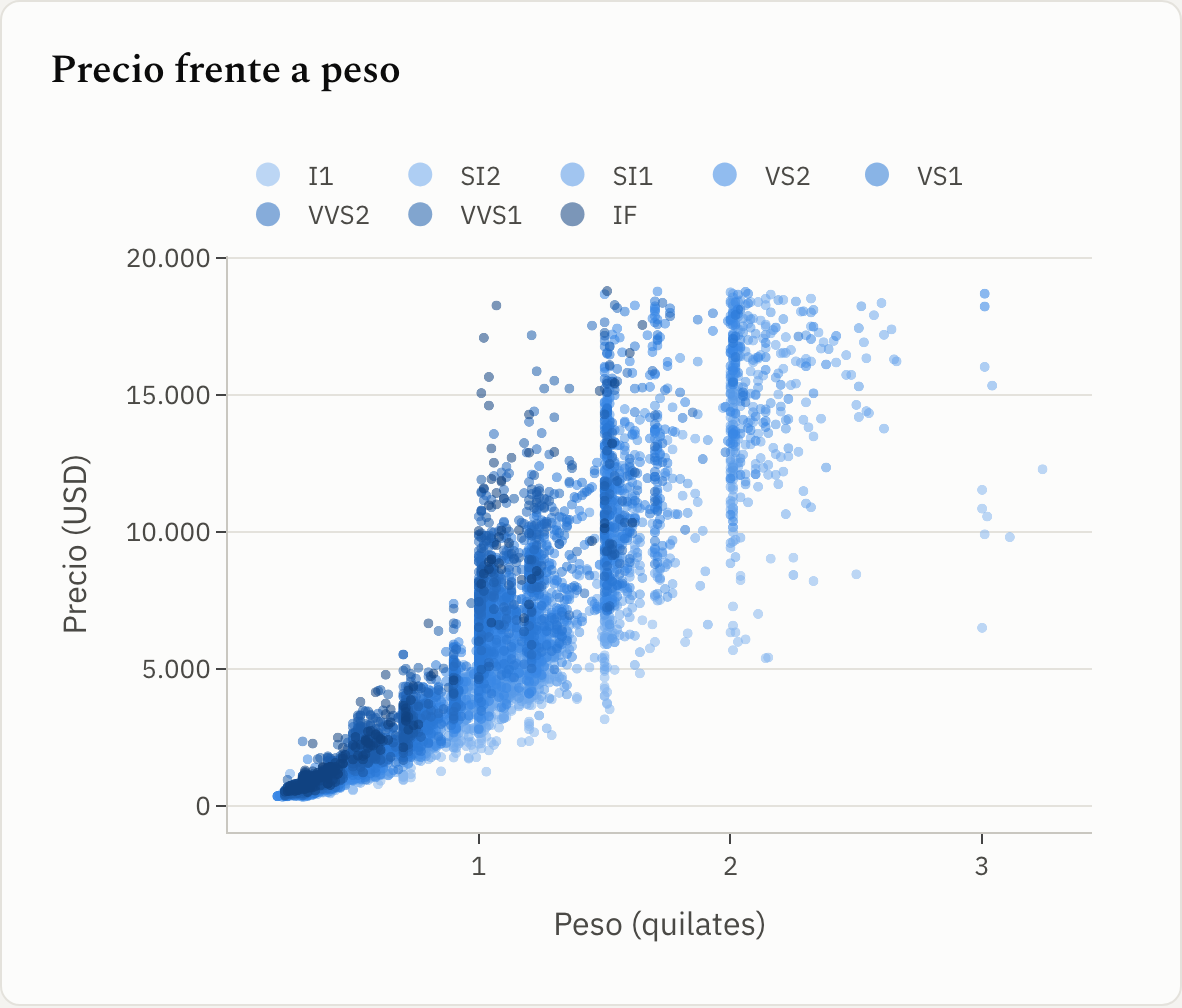
\includegraphics[width=\textwidth]{figuras/explorar-lineal}\\[-2pt]
{\small (a) Escala lineal: embudo y curvatura}
\end{minipage}\hfill
\begin{minipage}{0.49\textwidth}\centering
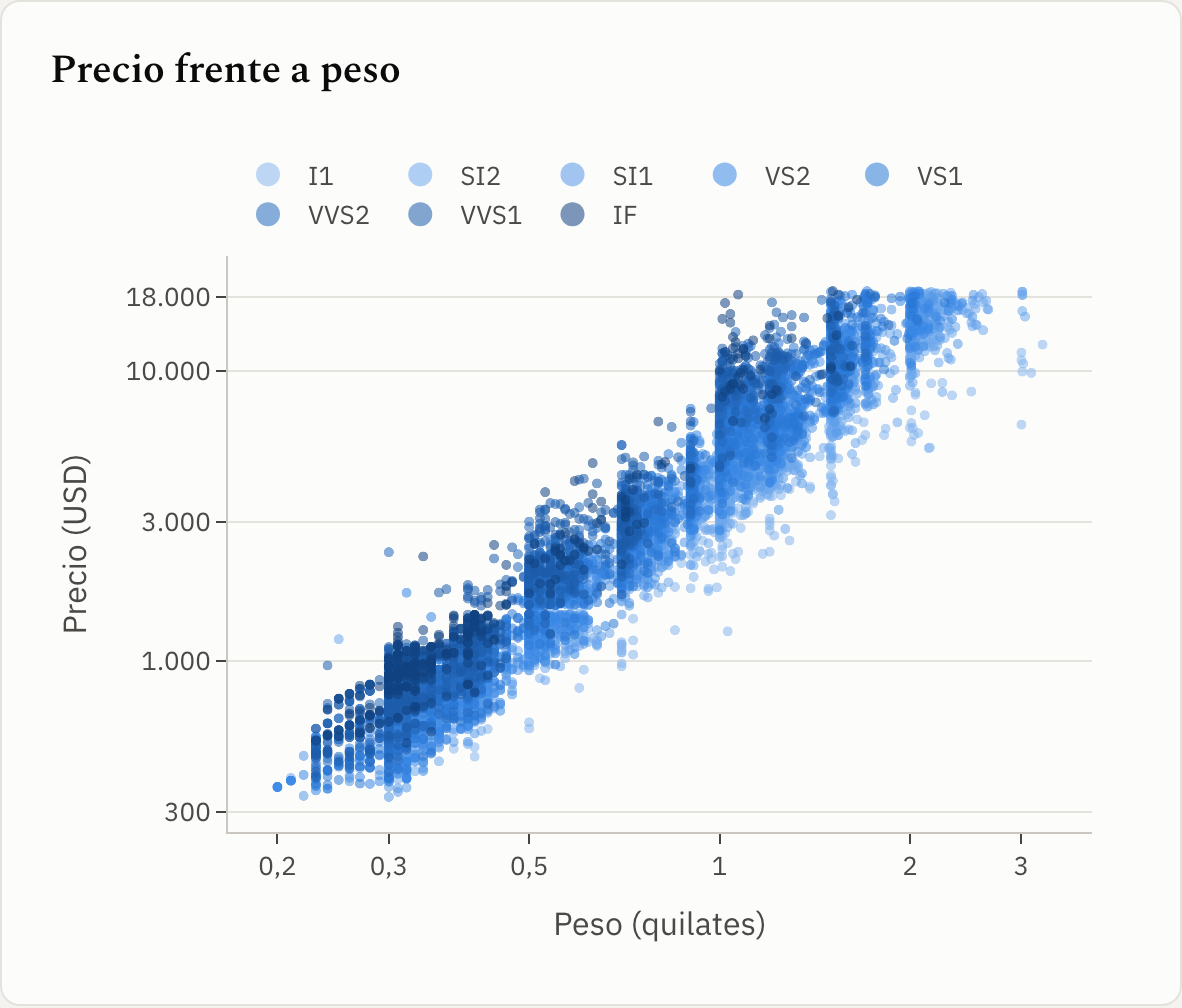
\includegraphics[width=\textwidth]{figuras/explorar-log}\\[-2pt]
{\small (b) Escala logarítmica: banda recta}
\end{minipage}
\caption{Precio frente a peso coloreado por pureza (pestaña 2 del dashboard, con el conmutador de escala). La forma de la nube justifica la transformación log-log de M3.}
\label{fig:loglog}
\end{figure}

\textbf{M4 y M5.} Se tratan en la sección~\ref{sec:hiper}: son la
experimentación con hiperparámetros y la regularización.

\section{Experimentación con hiperparámetros y regularización}\label{sec:hiper}

\subsection{Criterio de selección: regla de un error estándar}

En los dos barridos apliqué la misma regla: calcular el $R^2$ de validación
cruzada para cada valor del hiperparámetro y quedarme con el \textbf{modelo más
simple cuyo $R^2$ esté a menos de un error estándar del mejor}. Escoger el máximo
absoluto premia diferencias que están dentro del ruido de la validación y empuja
hacia modelos más complejos sin evidencia. Cada barrido varía una sola cosa y deja
el resto fijo, como en un experimento controlado.

\subsection{Regularización: Ridge y Lasso sobre M3 con interacciones}

M4 amplía M3 con todas las interacciones de grado 2 (189 términos): peso×color,
color×pureza, etc. Con tantos términos existe riesgo de sobreajuste, así que la
regresión se penaliza con Ridge (L2) y Lasso (L1), barriendo $\alpha$ en escala
logarítmica.

\begin{figure}[H]
\centering
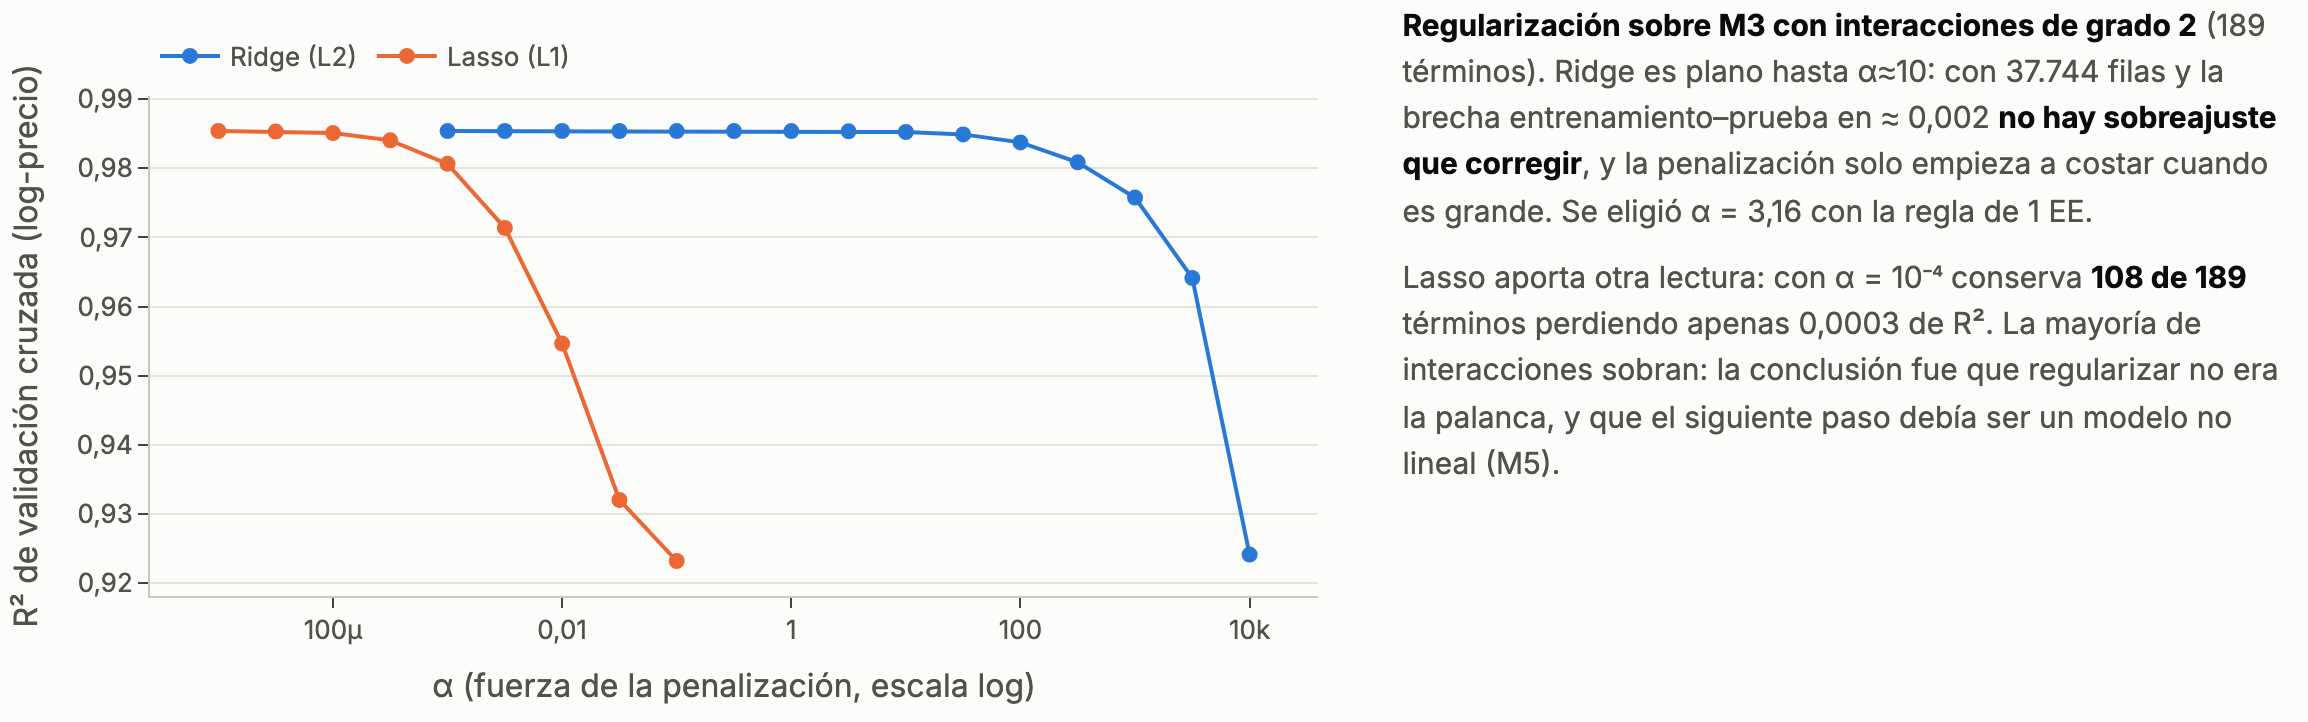
\includegraphics[width=\textwidth]{figuras/xp-alfa}
\caption{Barrido de $\alpha$ para Ridge y Lasso (captura del dashboard, pestaña 4).}
\end{figure}

\textbf{Resultado: no había sobreajuste que corregir.} La curva de Ridge es plana
hasta $\alpha \approx 10$ y solo empieza a caer con penalizaciones grandes. Con
37.744 filas para 189 términos, la brecha entre entrenamiento y validación es de
dos milésimas. La regla de un error estándar eligió $\alpha = 3{,}16$ y M4 mejora
a M3 en medio punto de $R^2$. Lasso aportó otra lectura: con $\alpha = 10^{-4}$
conserva solo \textbf{108 de los 189 términos} con una pérdida despreciable de
$R^2$. La mayoría de interacciones sobran. Conclusión: \emph{la regularización no
era la palanca}. El modelo lineal había llegado a su techo, y para bajar el error
hacía falta un modelo que aprendiera las interacciones por sí mismo.

\subsection{Profundidad del gradient boosting}

M5 es un \texttt{HistGradientBoostingRegressor} sobre log(precio) con todas las
variables, incluidas las medidas $x, y, z$. El hiperparámetro que controla el
sobreajuste es la profundidad de cada árbol. La barrí de 1 a 12 con el resto
fijo: 300 árboles y tasa de aprendizaje 0,1.

\begin{figure}[H]
\centering
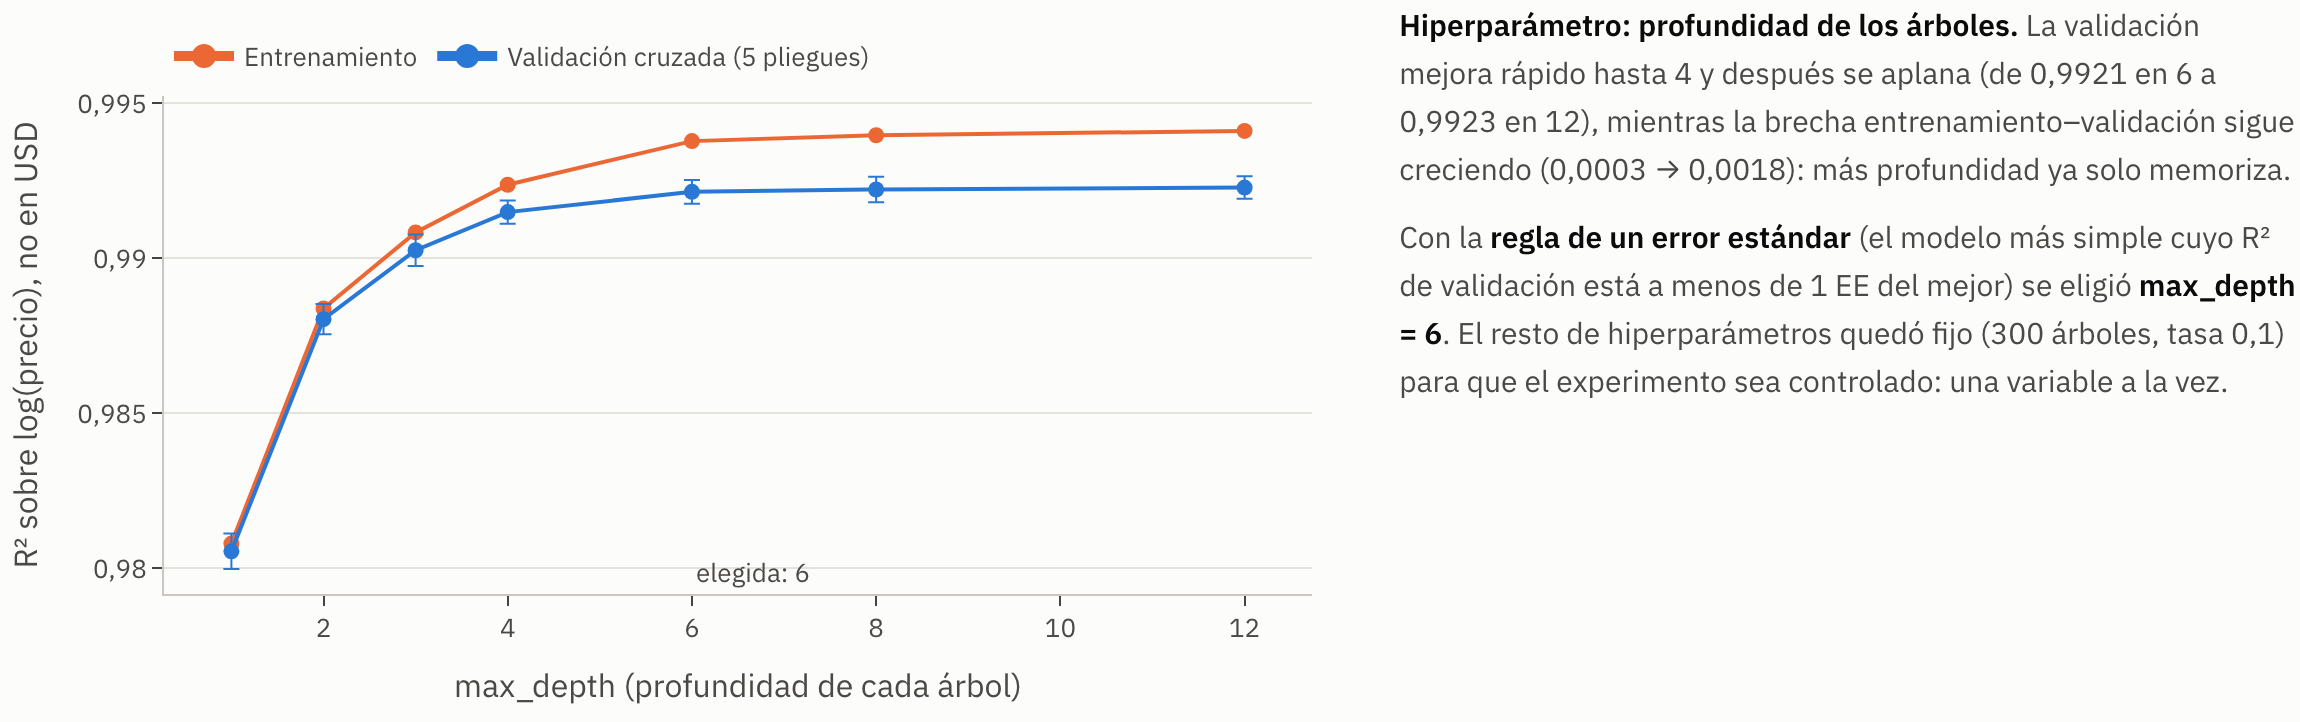
\includegraphics[width=\textwidth]{figuras/xp-profundidad}
\caption{$R^2$ de entrenamiento y de validación cruzada según la profundidad (pestaña 4 del dashboard).}
\end{figure}

La validación sube rápido hasta profundidad 4 y después se aplana: de 0,9921 en
6 a 0,9923 en 12. La brecha entre entrenamiento y validación, en cambio, sigue
creciendo, de 0,0003 a 0,0018. Pasada esa zona, más profundidad solo memoriza. La
regla de un error estándar eligió \texttt{max\_depth} = 6. En prueba, M5 alcanza
$R^2 = 0{,}9816$, RMSE de 535 USD y \textbf{MAPE de 6,5\,\%}, con una brecha
entrenamiento--prueba de 0,0047: el modelo generaliza.

\section{Calidad y cantidad de los datos}

\subsection{Una característica nueva y 20 registros defectuosos}

El catálogo trae 20 piedras con alguna dimensión en cero, algo físicamente
imposible. Probé una característica nueva, $\log(\text{volumen}) = \log(x \cdot y
\cdot z)$, de dos formas. La primera fue imputar los ceros con la mediana, que es
el atajo habitual: el $R^2$ \textbf{bajó} de 0,9612 a 0,9592. La segunda fue
eliminar esos 20 registros: el $R^2$ subió apenas a 0,9613. Veinte filas
defectuosas entre 53.940 (0,04\,\%) bastaron para anular la ganancia de una
característica. Por eso la limpieza se aplica antes de la partición en todos los
modelos. El volumen resultó casi redundante con el peso, porque la densidad del
diamante es constante, así que M3 no lo incluye.

\begin{figure}[H]
\centering
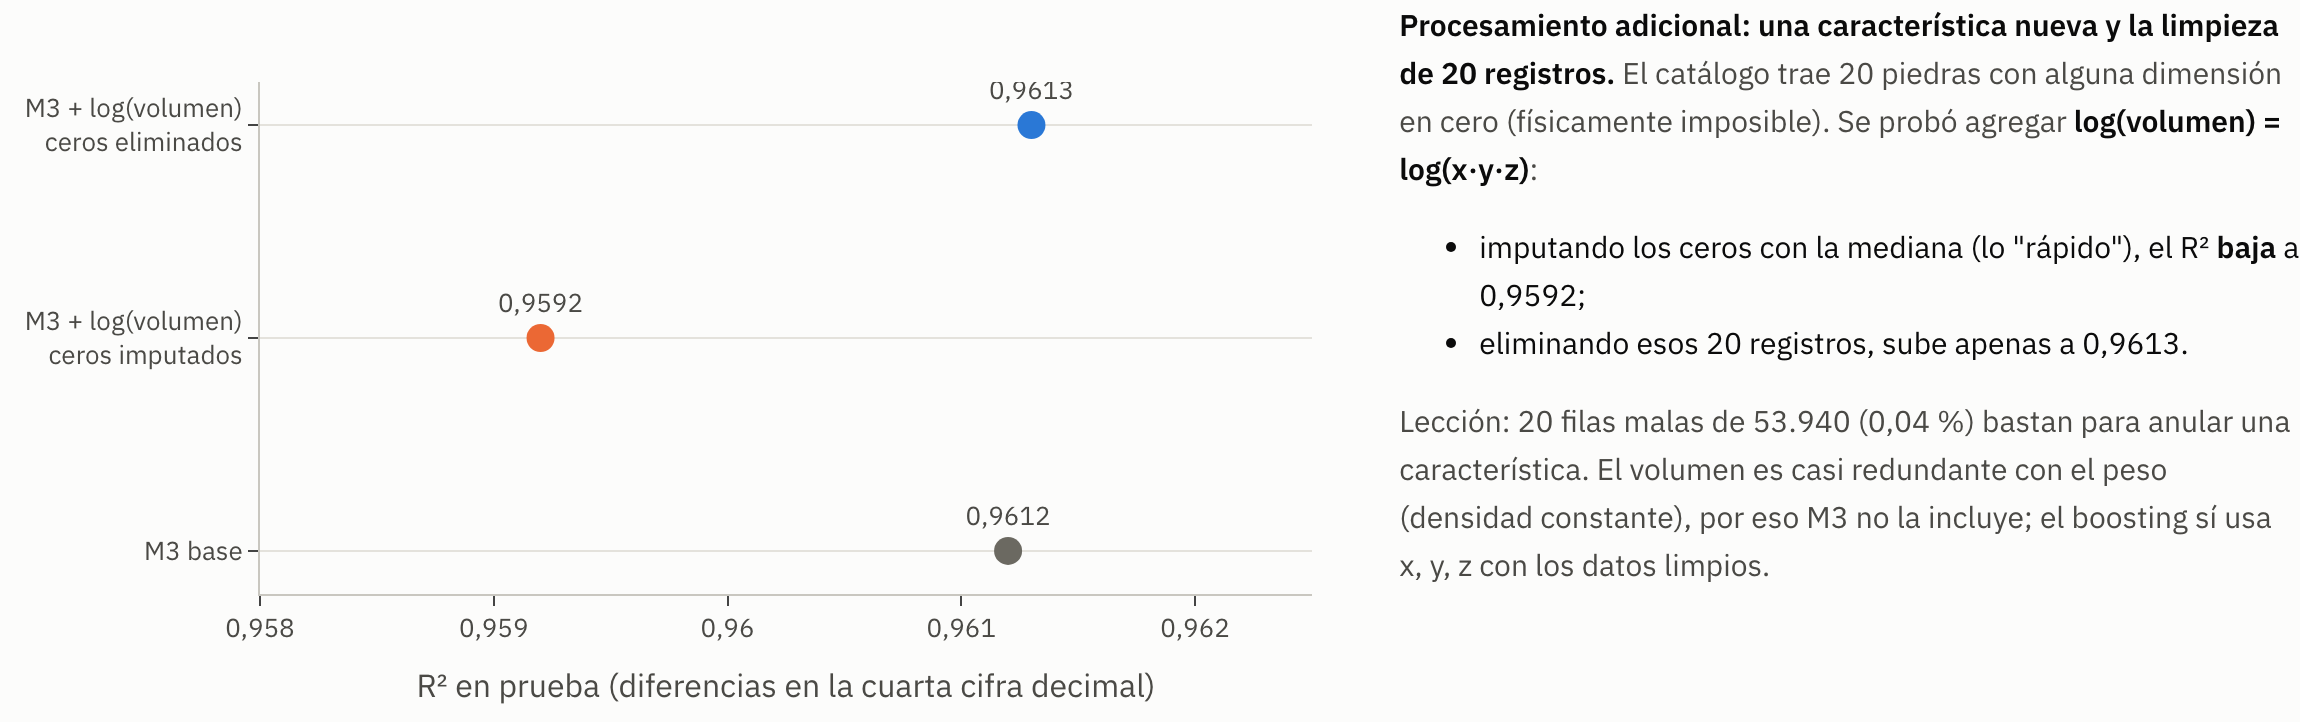
\includegraphics[width=\textwidth]{figuras/xp-calidad}
\caption{Experimento de calidad de datos (pestaña 4). Imputar los ceros con la mediana hunde el $R^2$ por debajo del modelo base; eliminarlos lo recupera. Las diferencias están en la cuarta cifra decimal, por eso se dibujan como puntos y no como barras con el eje truncado.}
\end{figure}

\subsection{¿Conseguir más datos ayudaría?}

Reentrené M3 y M5 con fracciones crecientes del entrenamiento (del 2\,\% al
100\,\%) y los medí siempre contra el mismo conjunto de prueba.

\begin{figure}[H]
\centering
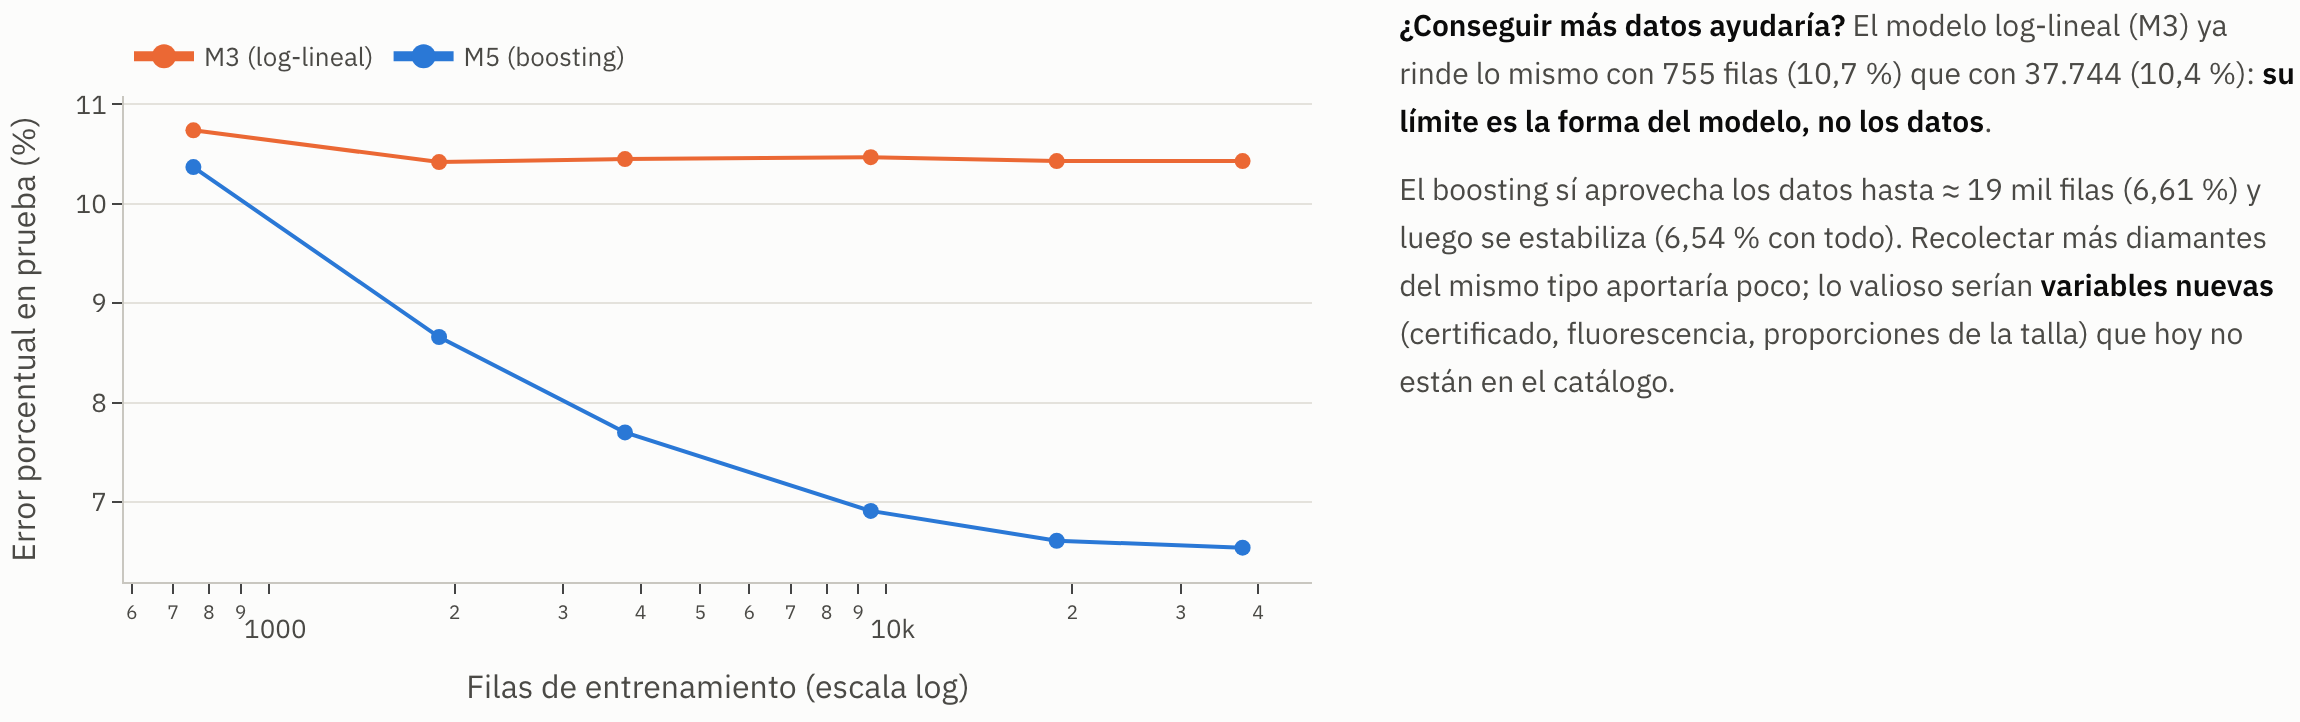
\includegraphics[width=\textwidth]{figuras/xp-curva}
\caption{Curva de aprendizaje: error porcentual en prueba según el tamaño del entrenamiento.}
\end{figure}

M3 rinde lo mismo con 755 filas (10,7\,\%) que con 37.744 (10,4\,\%): \textbf{su
límite es la forma del modelo, no la cantidad de datos}. M5 aprovecha los datos
hasta unas 19 mil filas (6,61\,\%) y luego se estabiliza. Recolectar más
diamantes del mismo tipo aportaría poco. Lo valioso sería recolectar
\textbf{variables nuevas}: laboratorio certificador, fluorescencia, proporciones
detalladas de la talla. Esa es la recomendación de recolección para la siguiente
versión.

\section{Fiabilidad del modelo final}

Para decidir si el modelo es fiable no basta un $R^2$ alto. Revisé tres cosas:

\begin{enumerate}[leftmargin=1.2cm,itemsep=0.2em]
\item \textbf{Generalización.} La brecha entre entrenamiento y prueba es de
0,0047 en $R^2$, y el gráfico de predicho frente a real (pestaña 4) sigue la
diagonal en todo el rango de precios, sin la curva ni el embudo de M1.

\begin{figure}[H]
\centering
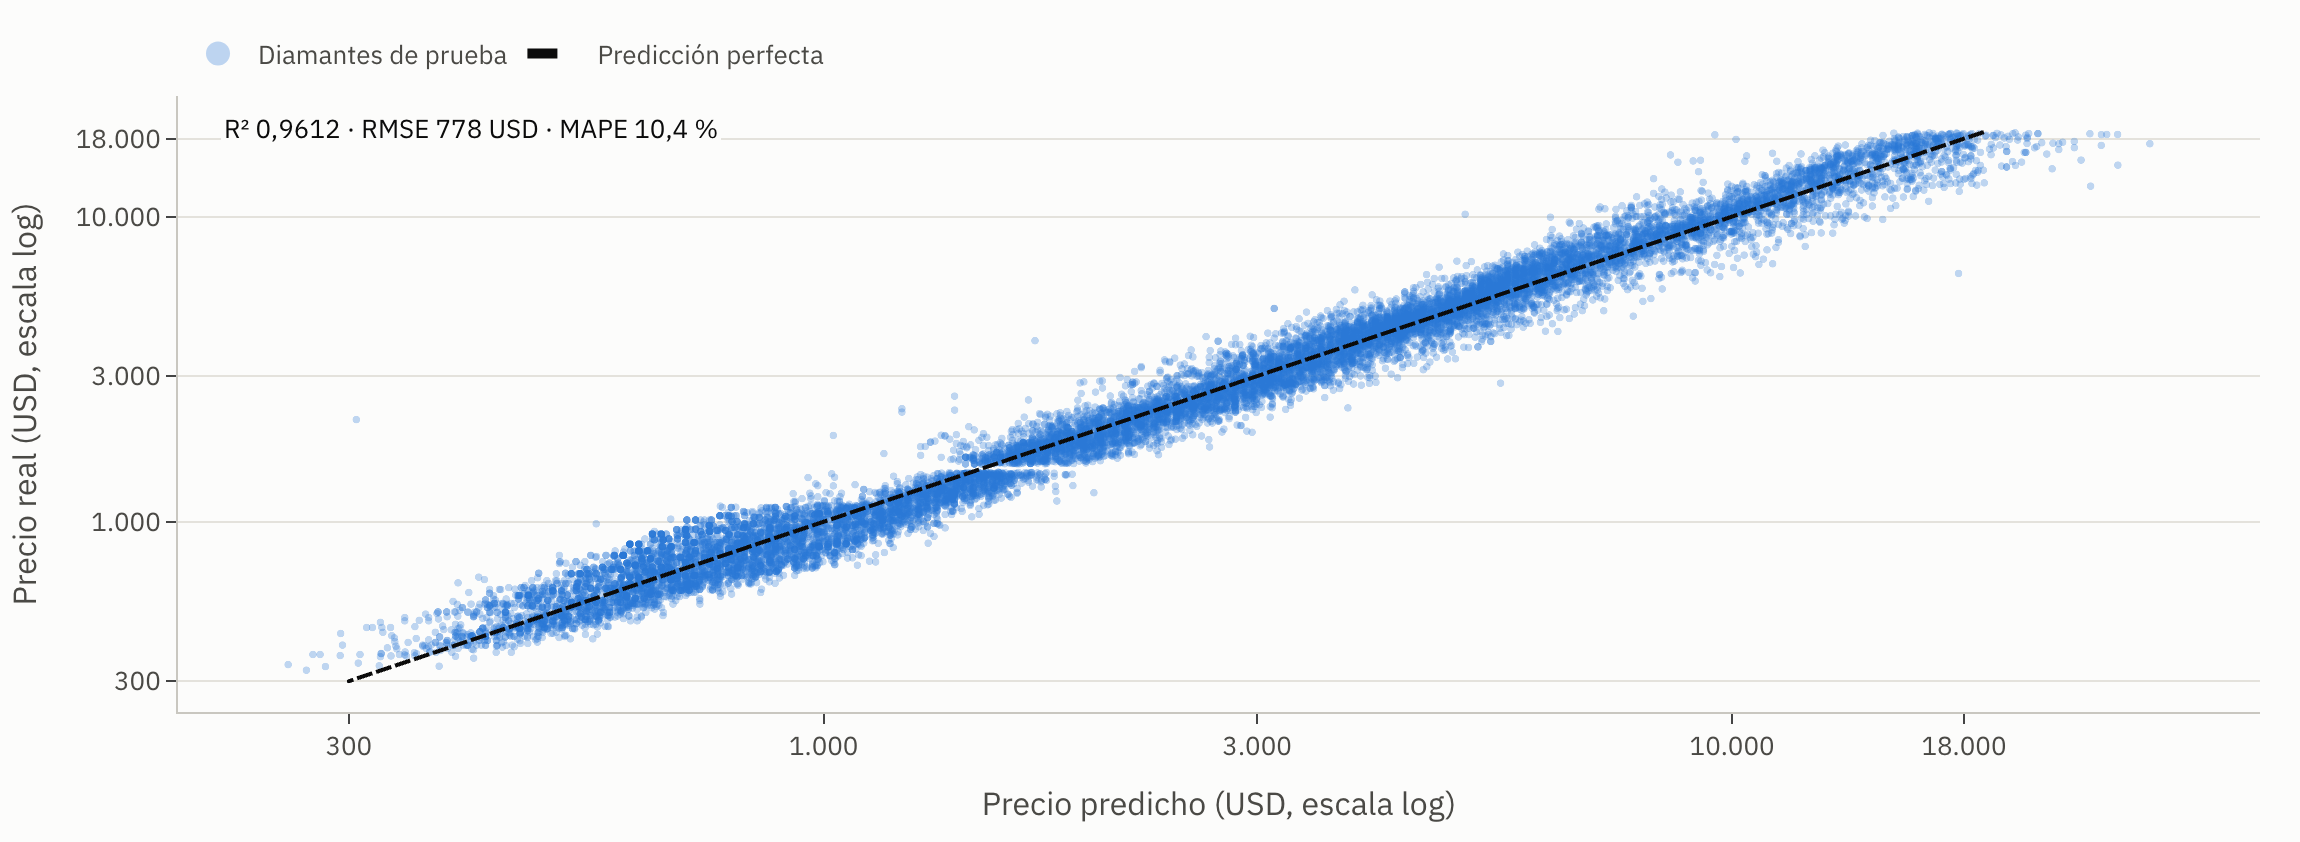
\includegraphics[width=\textwidth]{figuras/residuos-m3}\\[2pt]
{\small (a) M3, log-lineal: $R^2$ 0,9612 y MAPE 10,4\,\%}\\[6pt]
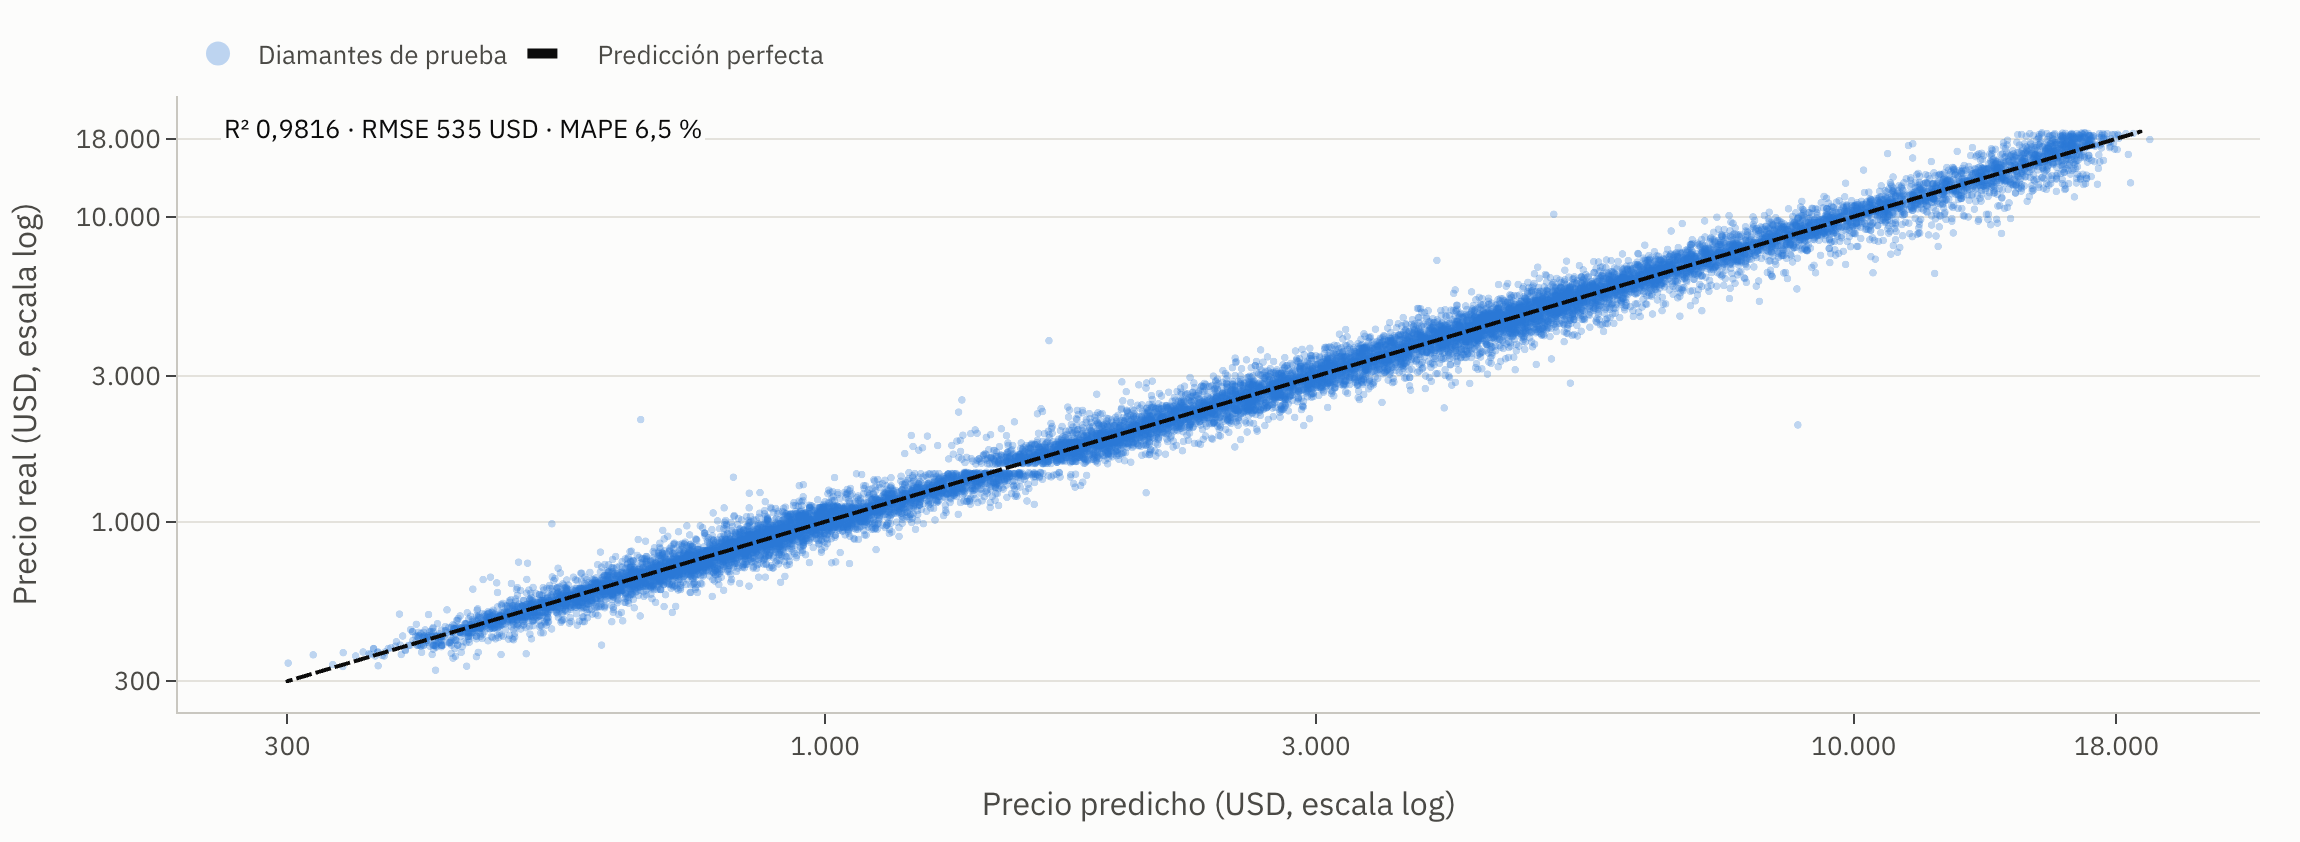
\includegraphics[width=\textwidth]{figuras/residuos-m5}\\[2pt]
{\small (b) M5, gradient boosting: $R^2$ 0,9816 y MAPE 6,5\,\%}
\caption{Precio predicho frente a real en los 16.176 diamantes de prueba, en escala logarítmica (pestaña 4). Ambos siguen la diagonal, pero M3 conserva un sesgo leve: según el tramo de precio predicho, su residuo mediano va de $-6{,}1$\,\% a $+4{,}1$\,\%. M5 lo reduce a menos de $\pm 1$\,\% y estrecha la nube, sobre todo en las piedras baratas: en el tercio de menor precio, el error típico baja de 12,2\,\% a 5,7\,\%.}
\end{figure}
\item \textbf{Incertidumbre honesta.} El tasador da un intervalo del 80\,\% en
lugar de un número suelto. Calibré el intervalo con los residuos \emph{fuera de
pliegue} del entrenamiento (\texttt{cross\_val\_predict}) y medí su cobertura en
prueba: \textbf{80,1\,\%}, que coincide con el valor nominal. El intervalo va de
$-9{,}9$\,\% a $+10{,}6$\,\% alrededor de la estimación. En una primera versión
calibré el intervalo con los residuos de prueba, pero así la cobertura da 80\,\%
por construcción y no demuestra nada. Lo corregí antes de publicar.
\item \textbf{Coherencia con el dominio.} Los efectos que estima M3 son
monótonos: cada escalón de color y de pureza suma prima. Esto resuelve la
paradoja de Simpson: a igual peso, corte y pureza, \textbf{D vale un 67\,\% más
que J}, aunque en bruto D promedie 3.168 USD y J 5.324 USD (los J pesan en
promedio 1,16 quilates y los D 0,66).
\end{enumerate}

\begin{figure}[H]
\centering
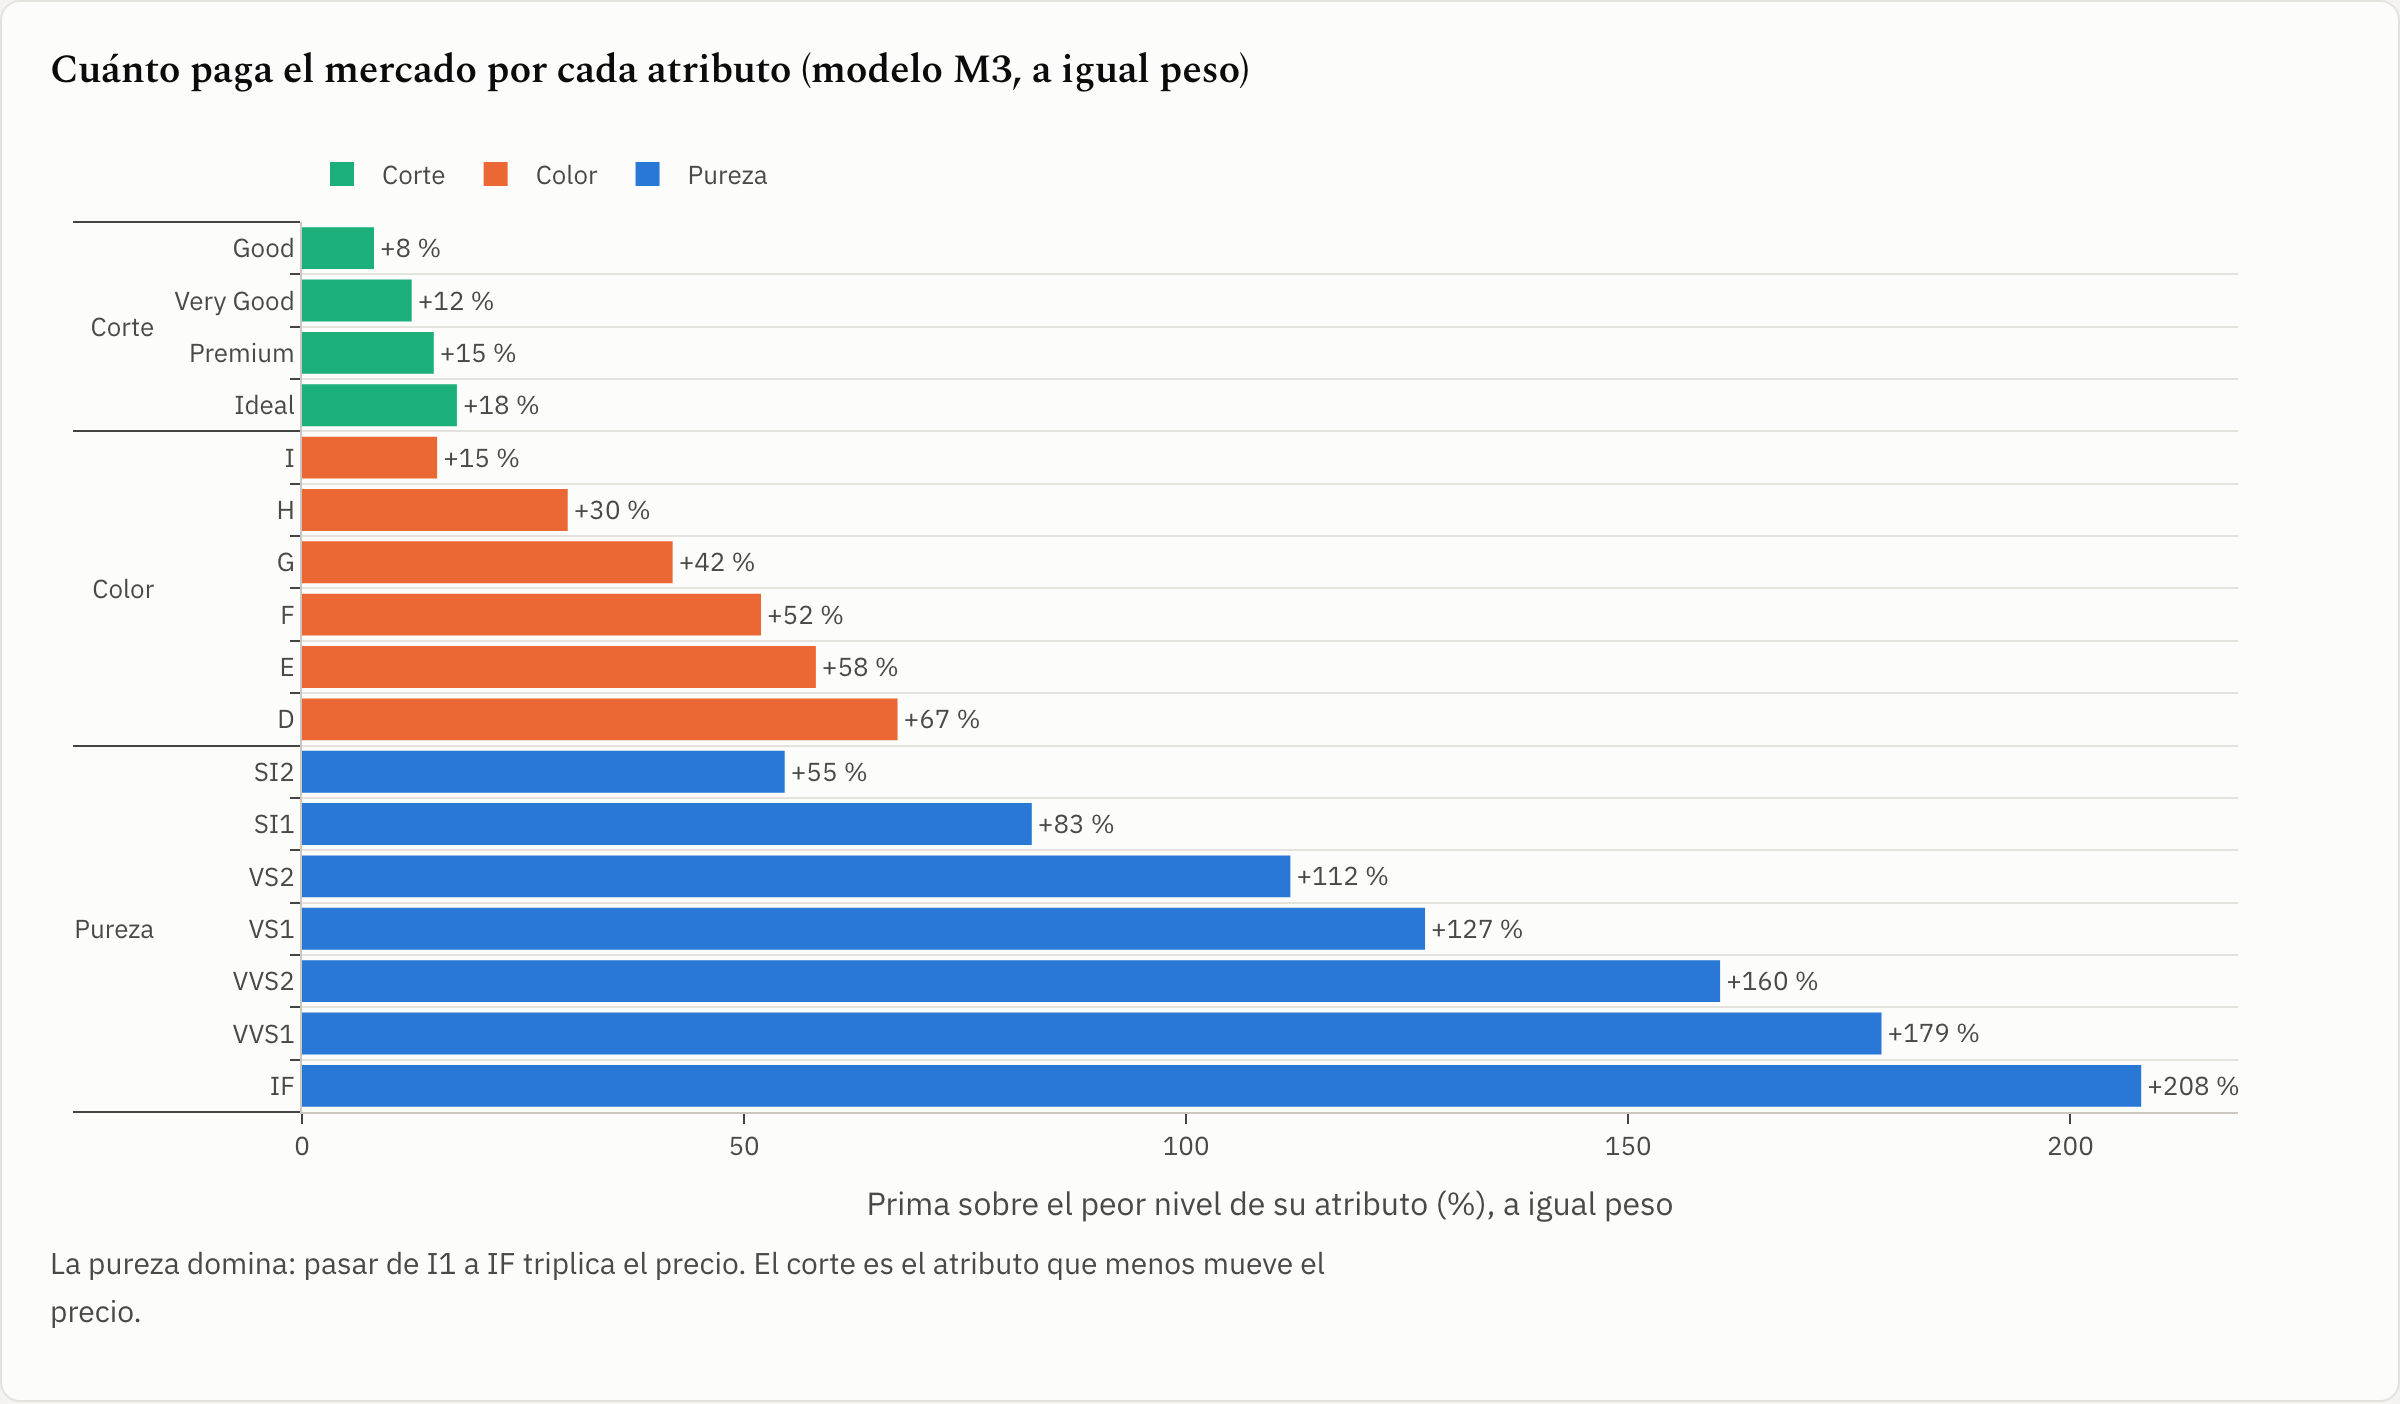
\includegraphics[width=0.92\textwidth]{figuras/efectos}
\caption{Prima que paga el mercado por cada nivel frente al peor de su atributo, a igual peso (coeficientes de M3, pestaña 3). Los efectos son monótonos dentro de cada atributo, y la pureza domina: IF vale un 208\,\% más que I1, mientras que el mejor corte solo suma un 18\,\%.}
\end{figure}

La Figura~\ref{fig:banda} comprueba la paradoja sin ningún modelo. Al comparar D
y J solo entre piedras de 0,3 a 0,5 quilates (pesos medios de 0,37 en ambos
colores), la distribución de D queda claramente a la derecha: D cuesta en
promedio 309 USD más, la misma cifra que obtuvo el contraste de hipótesis de la
actividad 4.

\begin{figure}[H]
\centering
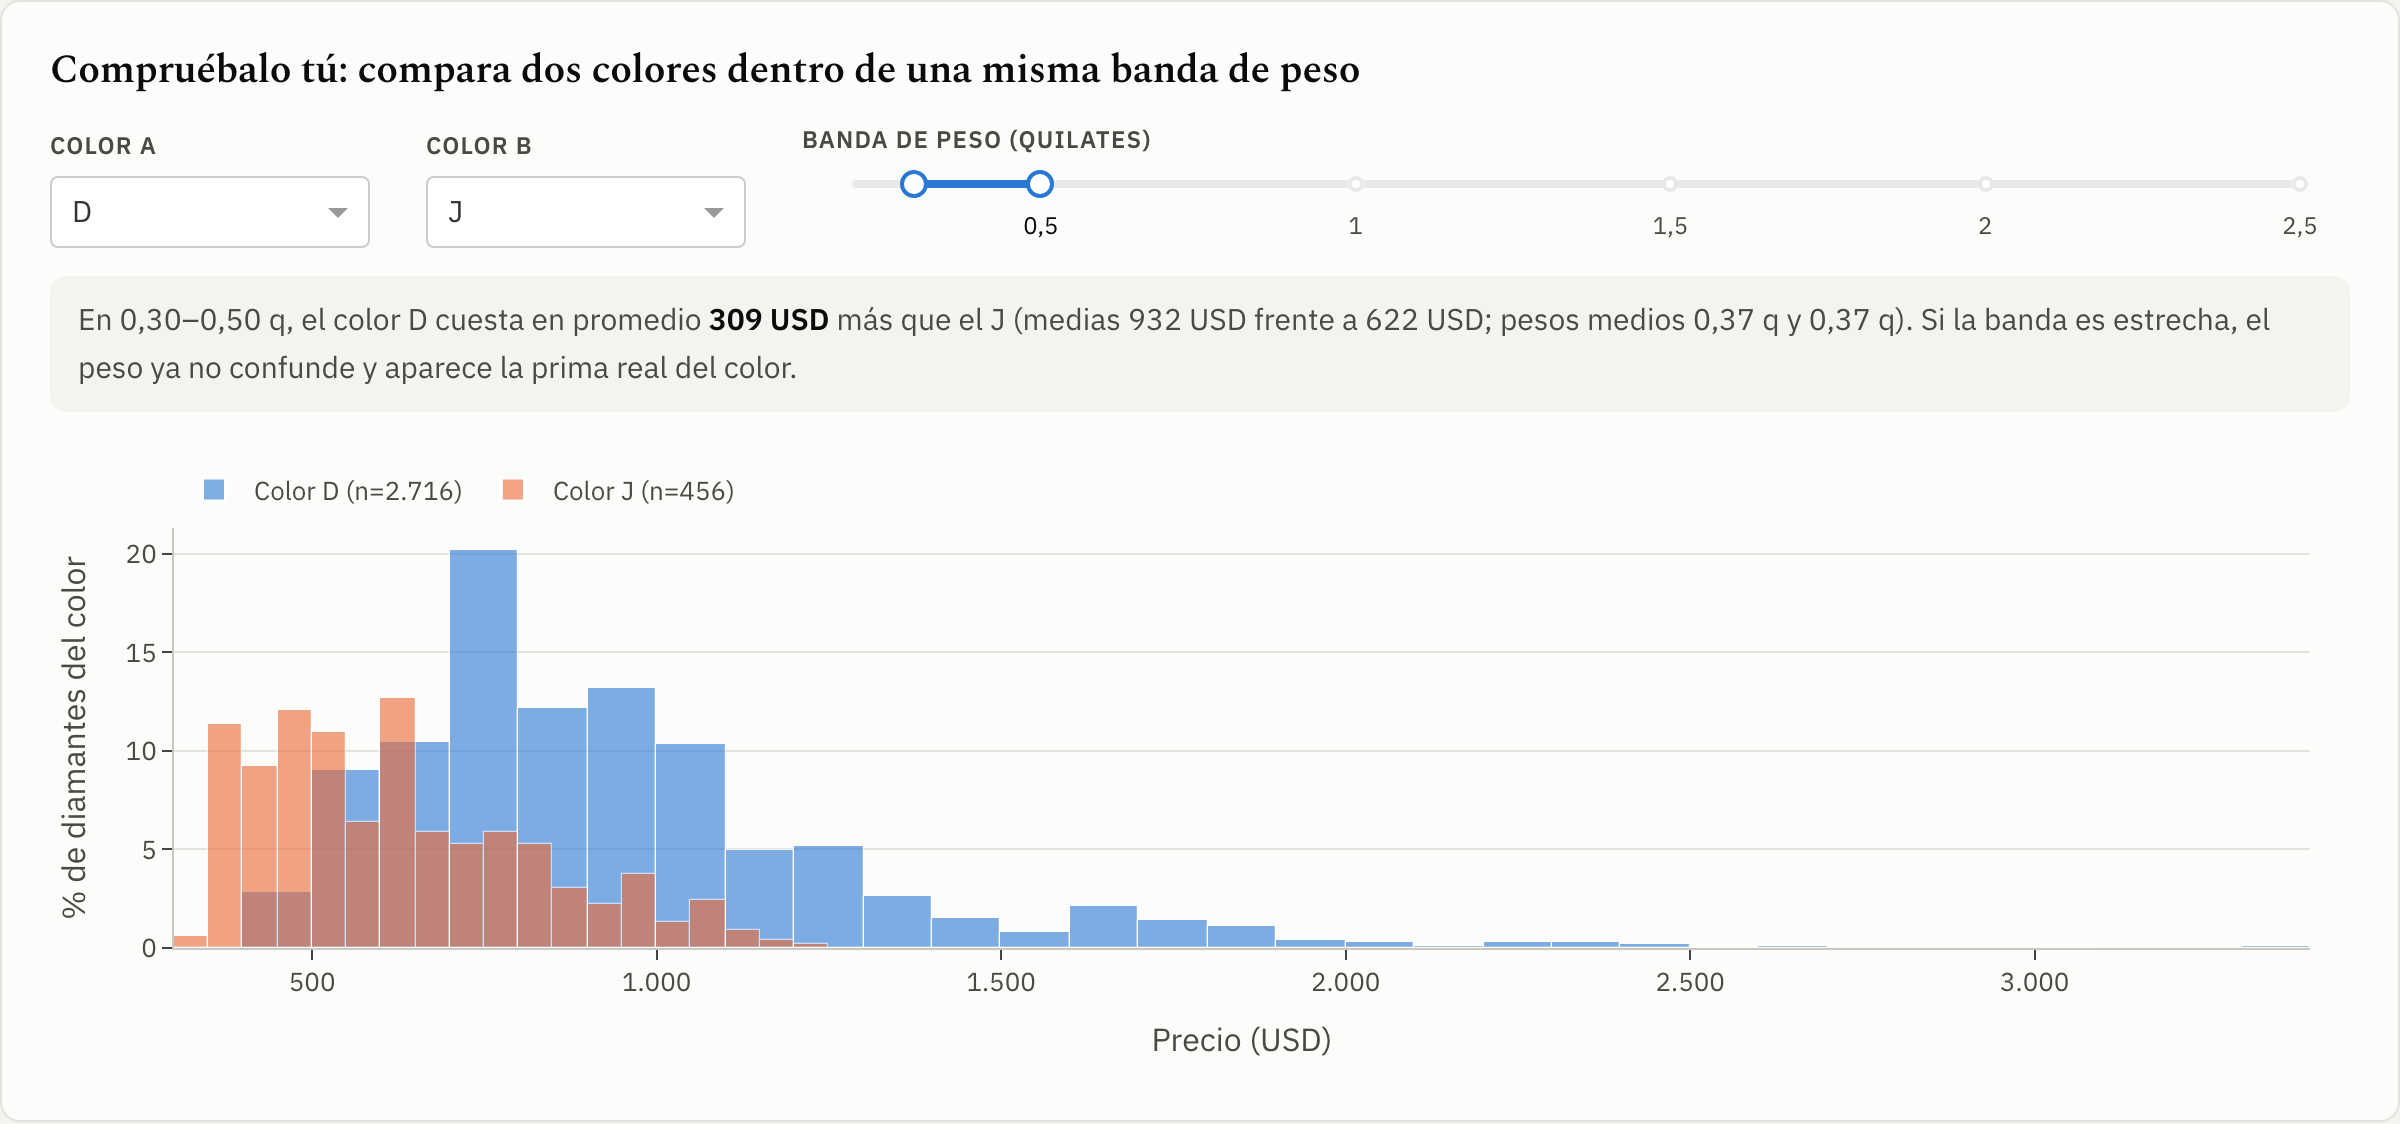
\includegraphics[width=\textwidth]{figuras/comprobar-banda}
\caption{Comparación interactiva de colores dentro de una banda de peso (pestaña 3). Con el peso controlado, el orden se endereza: D es más caro que J.}
\label{fig:banda}
\end{figure}

Con esta evidencia doy el modelo por fiable para su propósito: una primera
tasación automática con $\pm 10$\,\% de incertidumbre, que un tasador humano
revisa solo cuando el precio de lista se sale del intervalo.

\section{El dashboard}

\begin{figure}[H]
\centering

\includegraphics[width=\textwidth]{figuras/estructura}
\caption{Cabecera y navegación del dashboard: cinco pestañas que siguen el hilo del informe, de la historia al tasador.}
\end{figure}

\subsection{Decisiones de diseño}

\begin{itemize}[leftmargin=1.2cm,itemsep=0.25em]
\item \textbf{Tecnología.} Dash con Plotly y Pandas, según la guía de la
actividad. El dashboard (\texttt{app.py}) \textbf{no entrena nada al arrancar}:
lee los resultados que deja \texttt{modelo.py} en \texttt{resultados/}. Separar el
cálculo de la presentación hace que la carga en Binder tarde segundos y no los
tres minutos del entrenamiento.
\item \textbf{Estructura narrativa.} Cinco pestañas que siguen el hilo del
informe: la historia, explorar el catálogo, la paradoja del color, los
experimentos del modelo, y el tasador con el detector de oportunidades. Cada
gráfico va acompañado de un texto que dice qué mirar y qué concluir.
\item \textbf{Color con función.} Corte, color y pureza son variables ordinales,
así que se codifican con una rampa de un solo tono (azul claro = peor calidad,
azul oscuro = mejor) y no con colores arbitrarios. Las comparaciones entre dos
series (entrenamiento frente a validación, Ridge frente a Lasso) usan azul y
naranja, un par que se distingue también con daltonismo. En los gráficos de
barras, el gris es contexto y el azul marca lo que se debe mirar.
\item \textbf{Tipografía.} Spectral, una serifa de libro, para títulos y
cifras, que evoca un certificado de tasación; IBM Plex Sans para el texto y los
controles, con números tabulares en indicadores y tablas.
\item \textbf{Formato local.} Coma decimal y punto de miles en ejes, tablas y
textos.
\item \textbf{Rendimiento.} El gráfico de dispersión usa WebGL
(\texttt{Scattergl}) y, si el filtro supera 12.000 puntos, dibuja una muestra
aleatoria. El panel lo avisa en su resumen.
\end{itemize}

\begin{figure}[H]
\centering
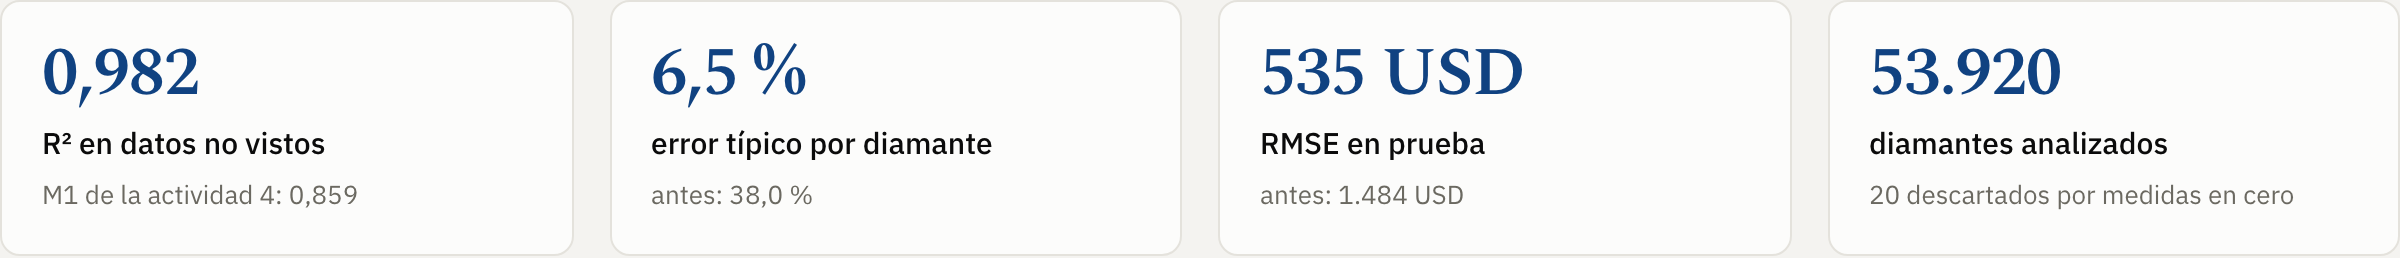
\includegraphics[width=\textwidth]{figuras/kpis}\\[4pt]
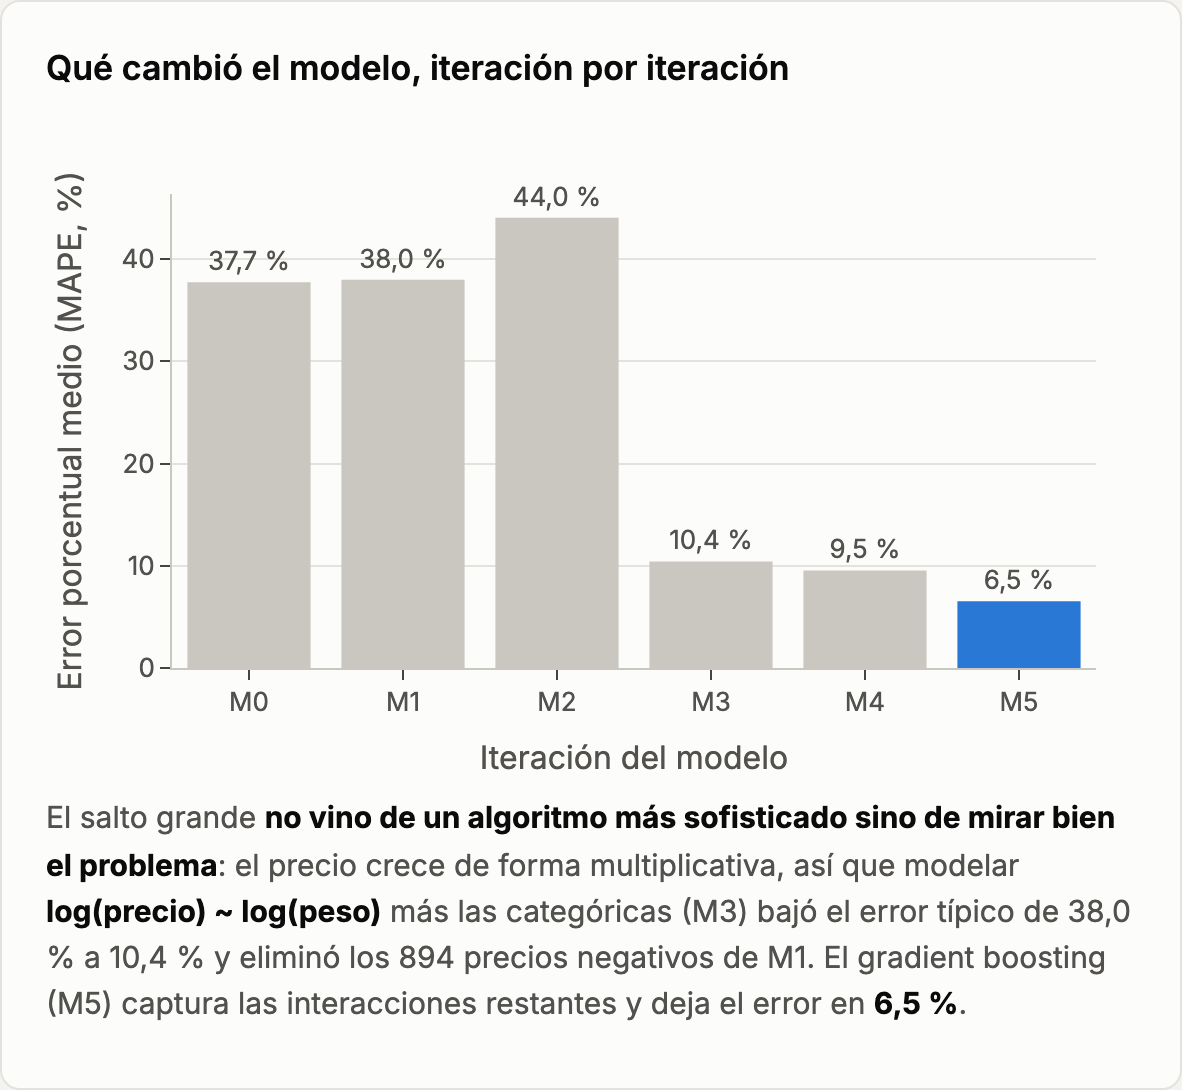
\includegraphics[width=0.62\textwidth]{figuras/evolucion}
\caption{Pestaña 1: indicadores y evolución del error en cada iteración.}
\end{figure}

Para un público que no es de joyería ni de estadística, la pestaña 1 cierra con
una guía de lectura (Figura~\ref{fig:guia}). Presenta las tres escalas
gemológicas como bandas ordenadas, con la misma rampa de azules que usan los
gráficos, y define las métricas. También aclara una confusión que detectó la
revisión de diseño: el $R^2$ de la pestaña 4 ($\approx$ 0,99) se mide sobre
log(precio), y el $R^2$ en dólares es 0,982.

\begin{figure}[H]
\centering
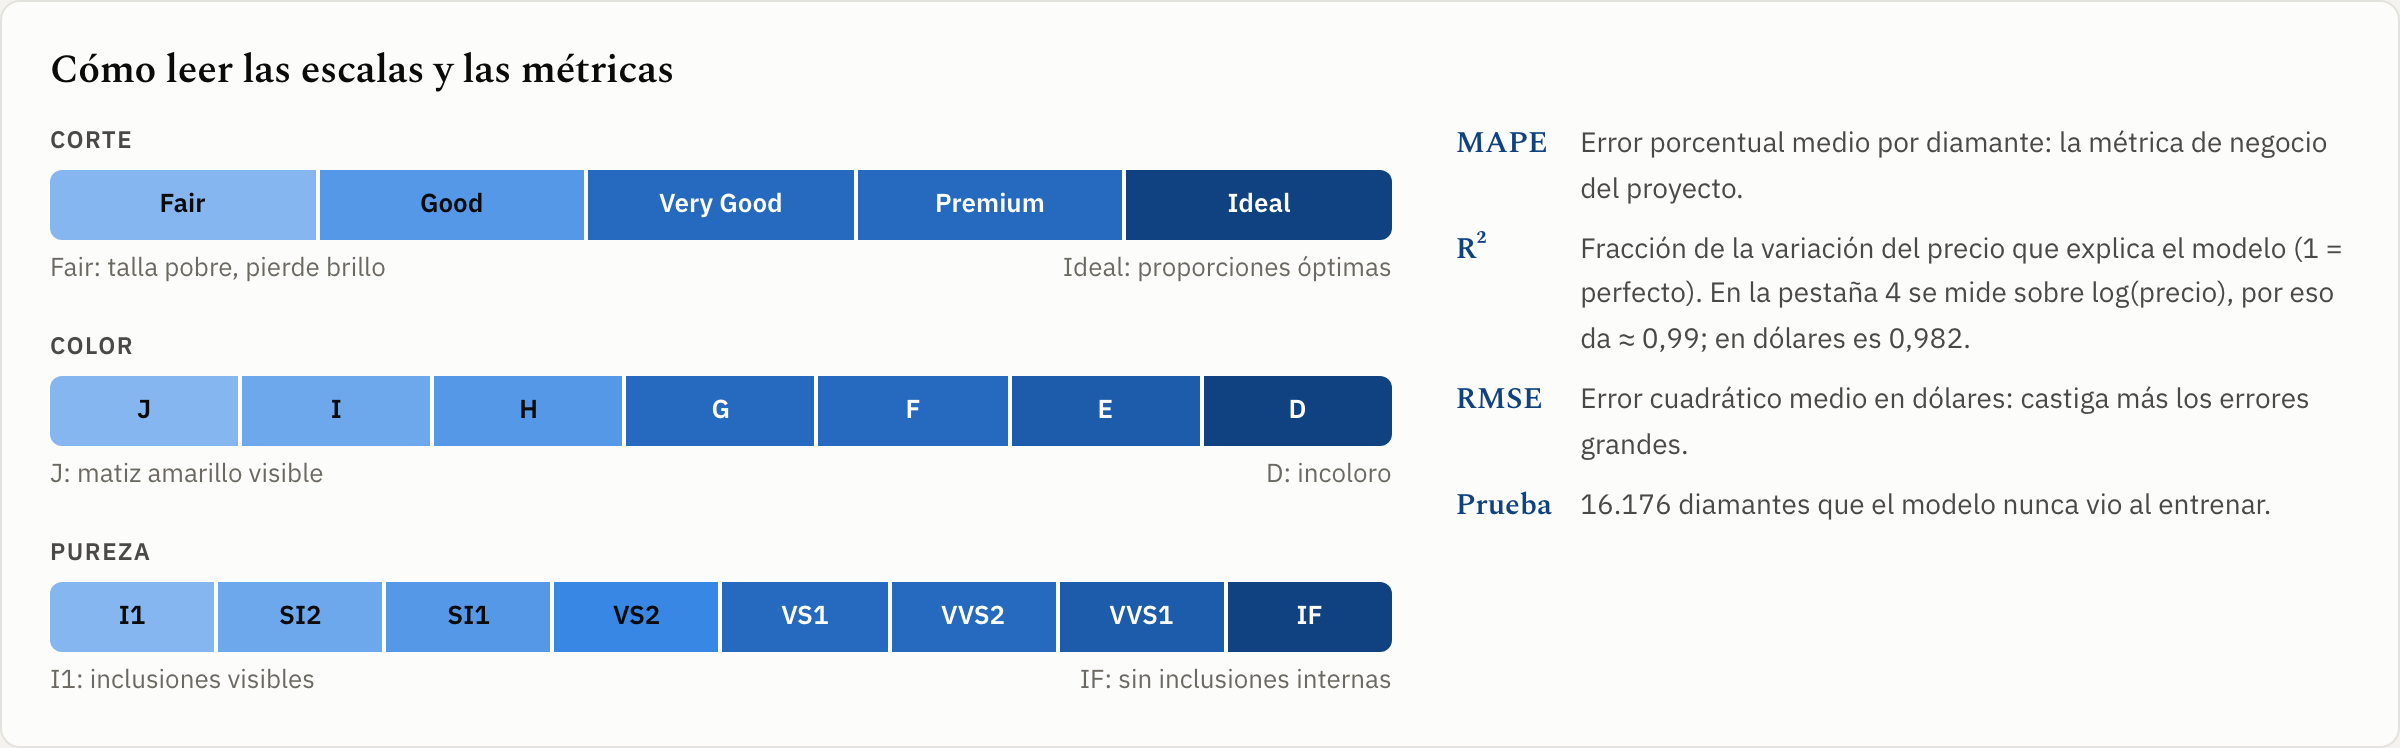
\includegraphics[width=\textwidth]{figuras/guia}
\caption{Guía de escalas y métricas (pestaña 1).}
\label{fig:guia}
\end{figure}

\subsection{Interactividad}

\begin{itemize}[leftmargin=1.2cm,itemsep=0.25em]
\item \textbf{Explorar el catálogo.} Filtro por corte (selección múltiple), rango
de peso, variable de color (corte, color o pureza) y escala lineal o logarítmica.
Al cambiar la escala se ve por qué se eligió la transformación log-log: la nube
se convierte en una banda recta.
\item \textbf{La paradoja del color.} El usuario elige dos colores y una banda de
peso, y el panel recalcula en vivo la diferencia de precios. Si la banda es
estrecha, el confusor desaparece y aparece la prima real del color.
\item \textbf{Experimentos.} Un selector recorre los cuatro experimentos:
profundidad, regularización, cantidad de datos y calidad de datos. Cada uno trae
su gráfico y su interpretación. Otro selector compara el predicho frente a real
de M3 y de M5.
\item \textbf{Tasador.} Peso, corte, color y pureza producen el precio estimado,
su intervalo del 80\,\% y un análisis de sensibilidad: cuánto cambia el precio al
mover un solo atributo.
\end{itemize}

\begin{figure}[H]
\centering
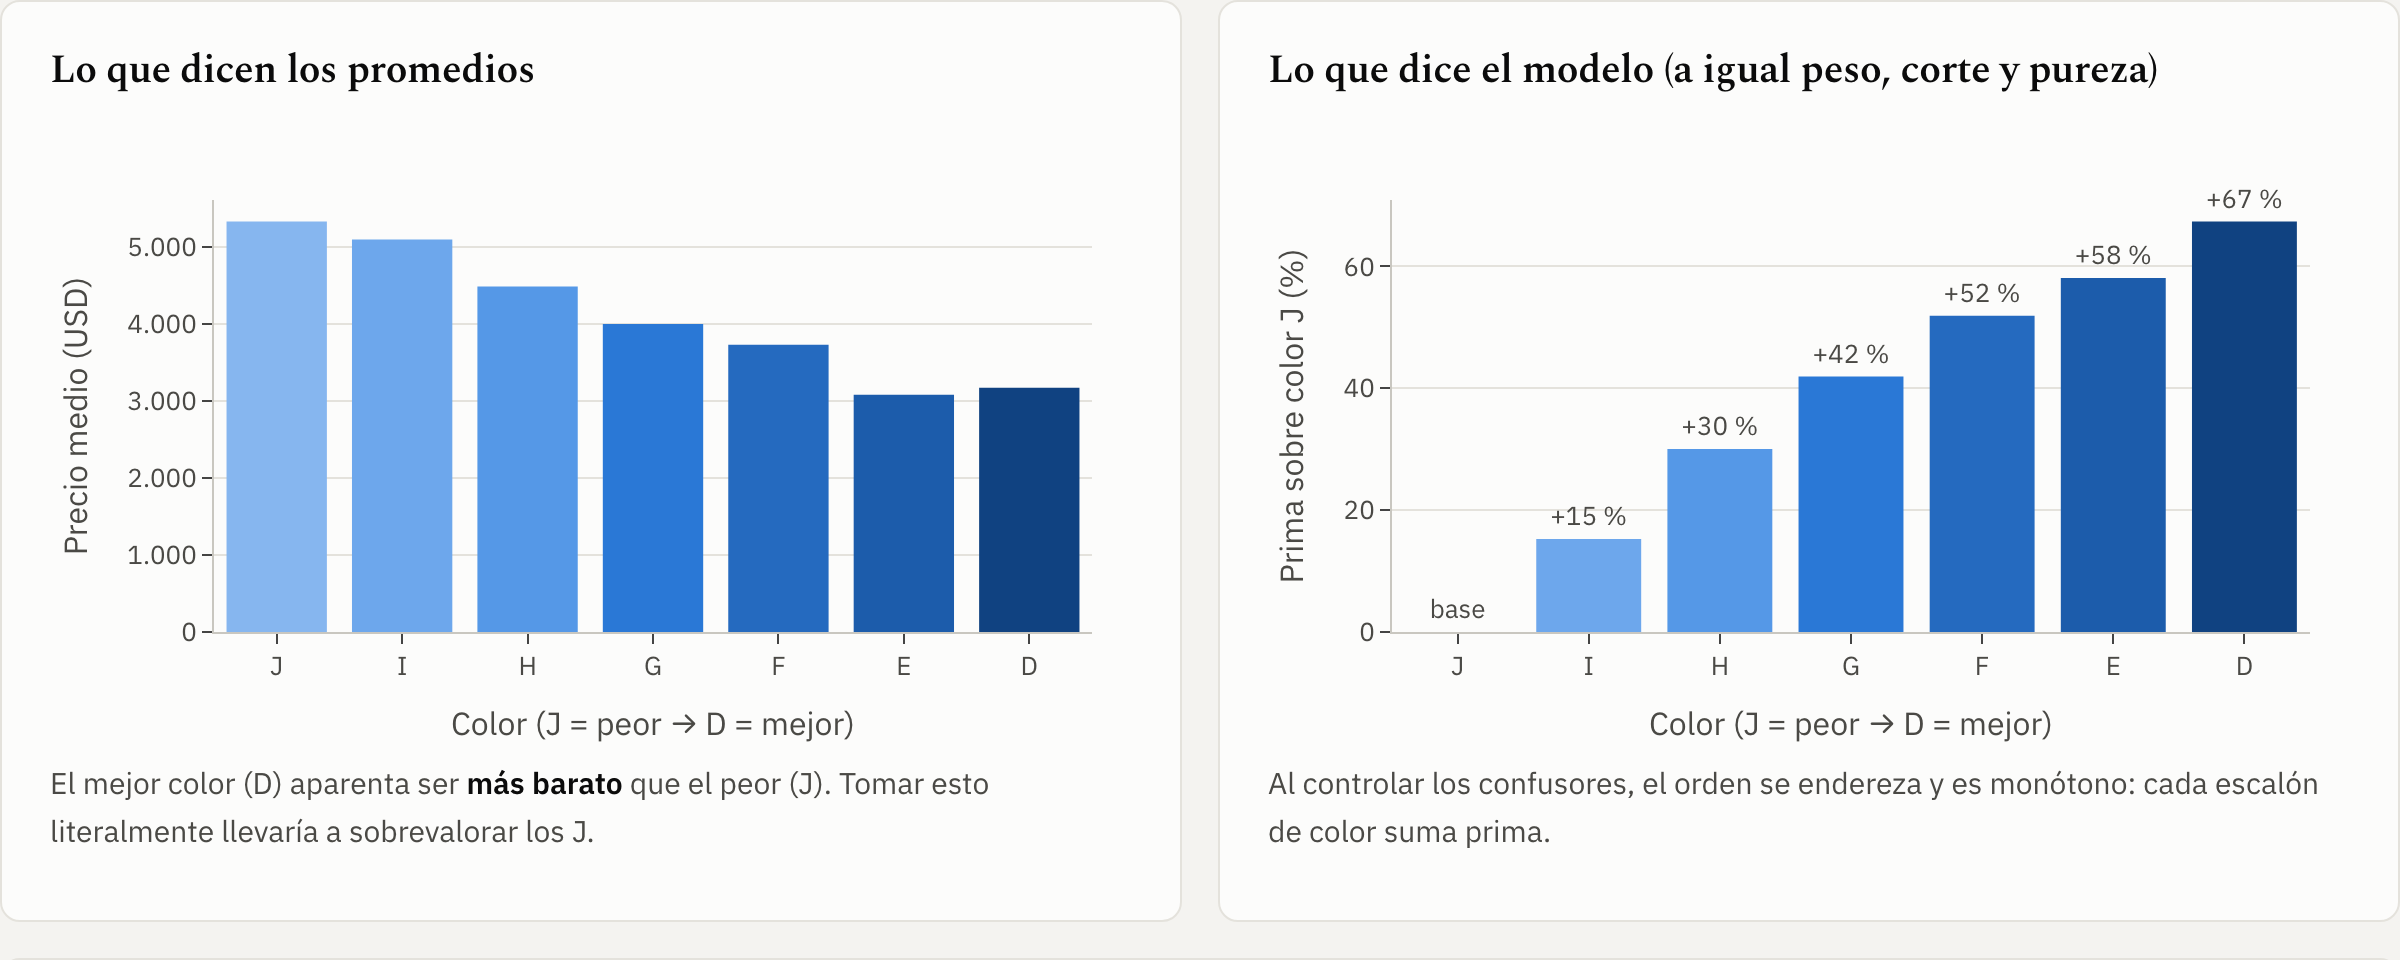
\includegraphics[width=\textwidth]{figuras/paradoja}
\caption{Pestaña 3: lo que dicen los promedios frente a lo que dice el modelo.}
\end{figure}

\subsection{Aporte original: el detector de oportunidades}

El modelo no solo tasa: también encuentra \textbf{piedras mal preciadas}. El
detector recorre los diamantes del conjunto de prueba, que el modelo nunca vio, y
lista los que tienen un precio de lista muy por debajo de lo que vale su
combinación de atributos, filtrando por presupuesto y descuento mínimo. En todo
el conjunto de prueba hay 255 diamantes a más de 20\,\% por debajo de su valor
estimado. Para una joyería compradora es una lista de revisión; para una
vendedora, una alerta de precios mal fijados. Los desvíos extremos (más del
50\,\%) se señalan para revisión manual, porque pueden ser errores de captura en
el catálogo.

\begin{figure}[H]
\centering
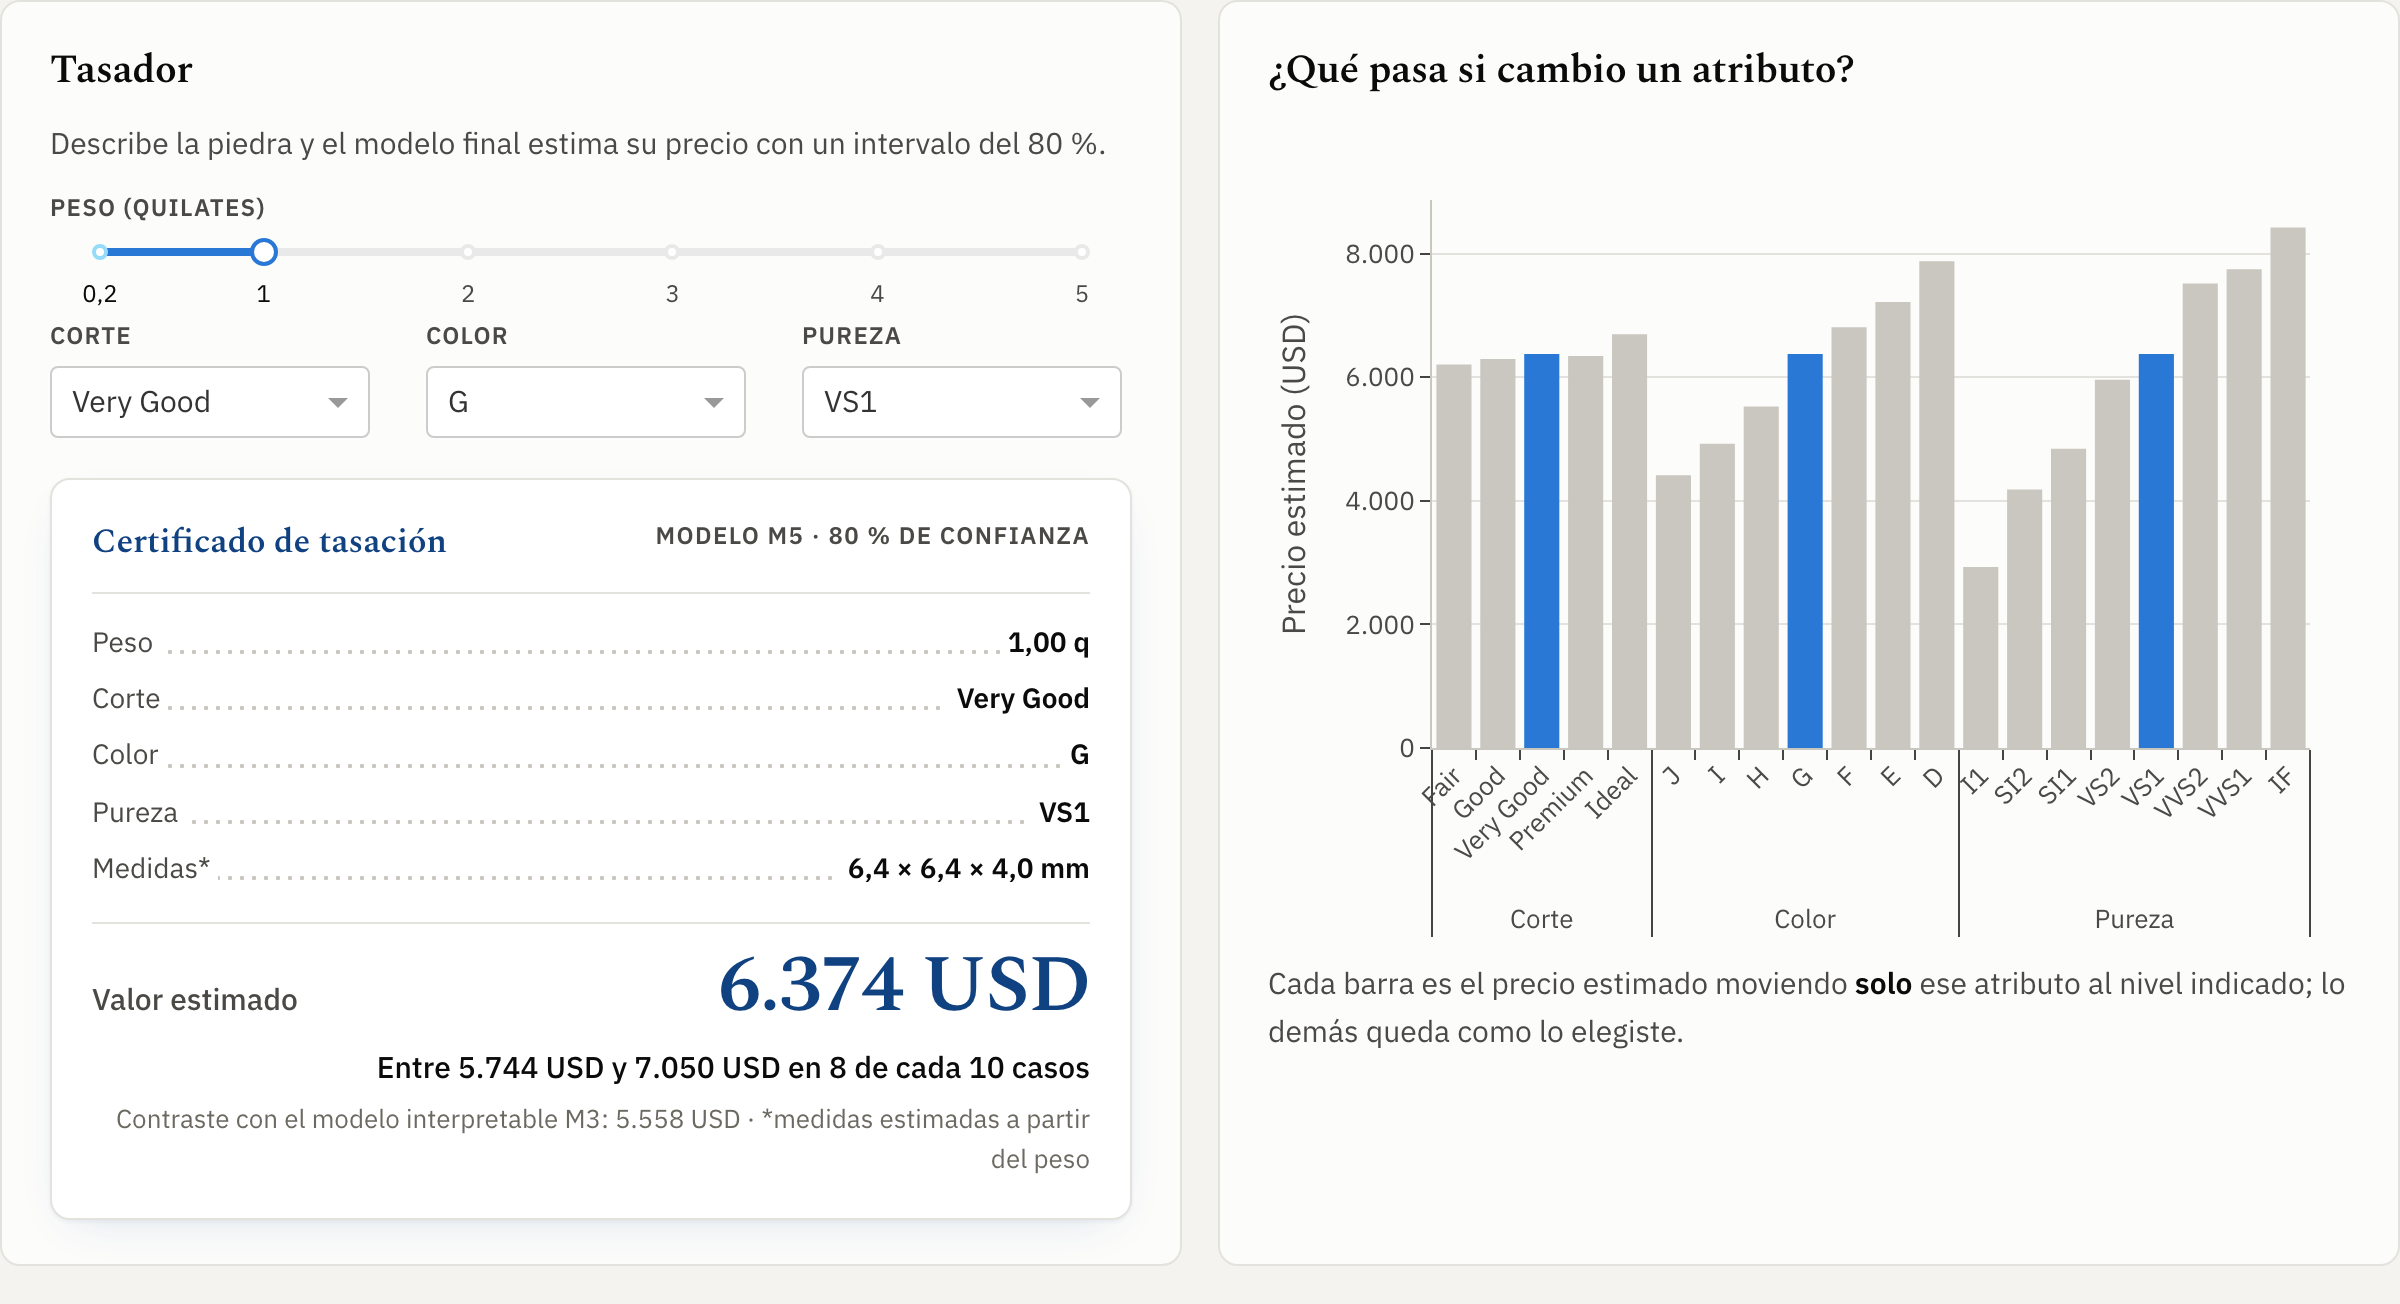
\includegraphics[width=\textwidth]{figuras/tasador}
\caption{Pestaña 5: tasador con intervalo y análisis de sensibilidad.}
\end{figure}

\begin{figure}[H]
\centering
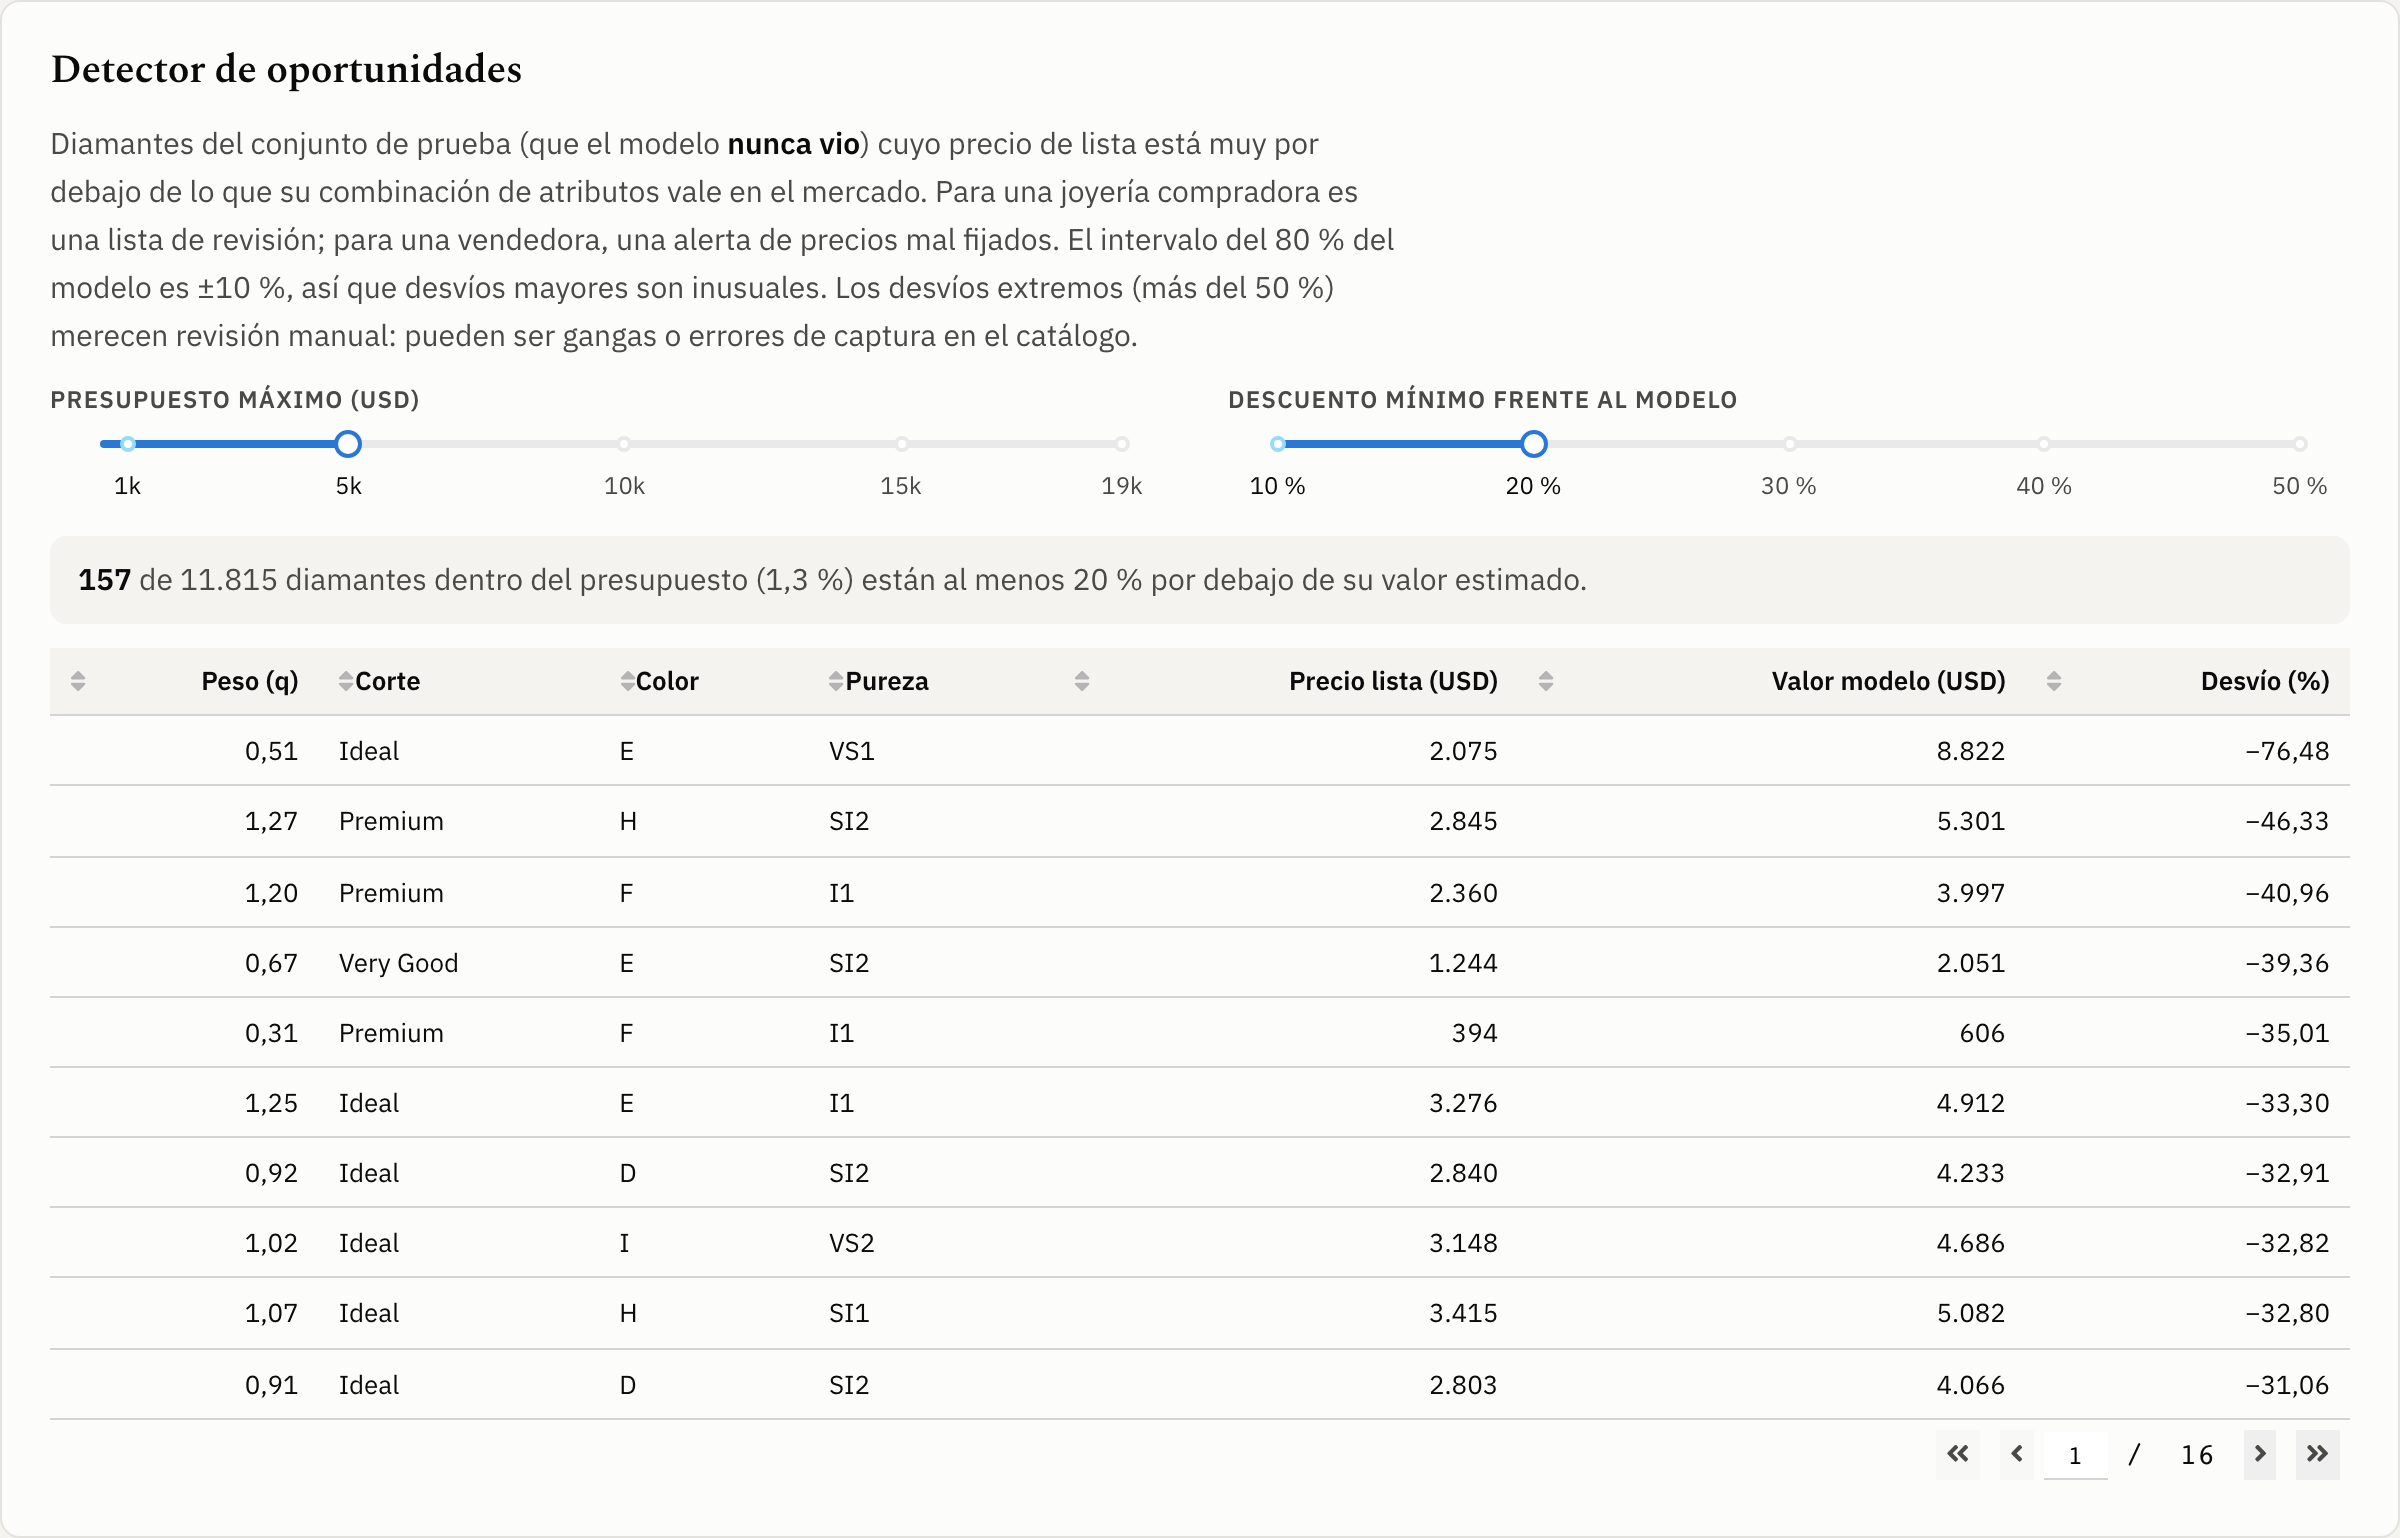
\includegraphics[width=\textwidth]{figuras/oportunidades}
\caption{Pestaña 5: detector de oportunidades.}
\end{figure}

\subsection{Estados vacíos y diseño adaptable}

Un filtro puede dejar el gráfico sin datos, por ejemplo al quitar todos los
cortes o al elegir una banda de peso sin diamantes de algún color. En ese caso
el dashboard no dibuja ejes rotos: muestra un mensaje que dice qué pasó y cómo
salir (Figura~\ref{fig:vacio}). Los rangos de los deslizadores no se pueden
cruzar, y la comparación de colores pide dos colores distintos.

\begin{figure}[H]
\centering
\begin{minipage}{0.62\textwidth}\centering
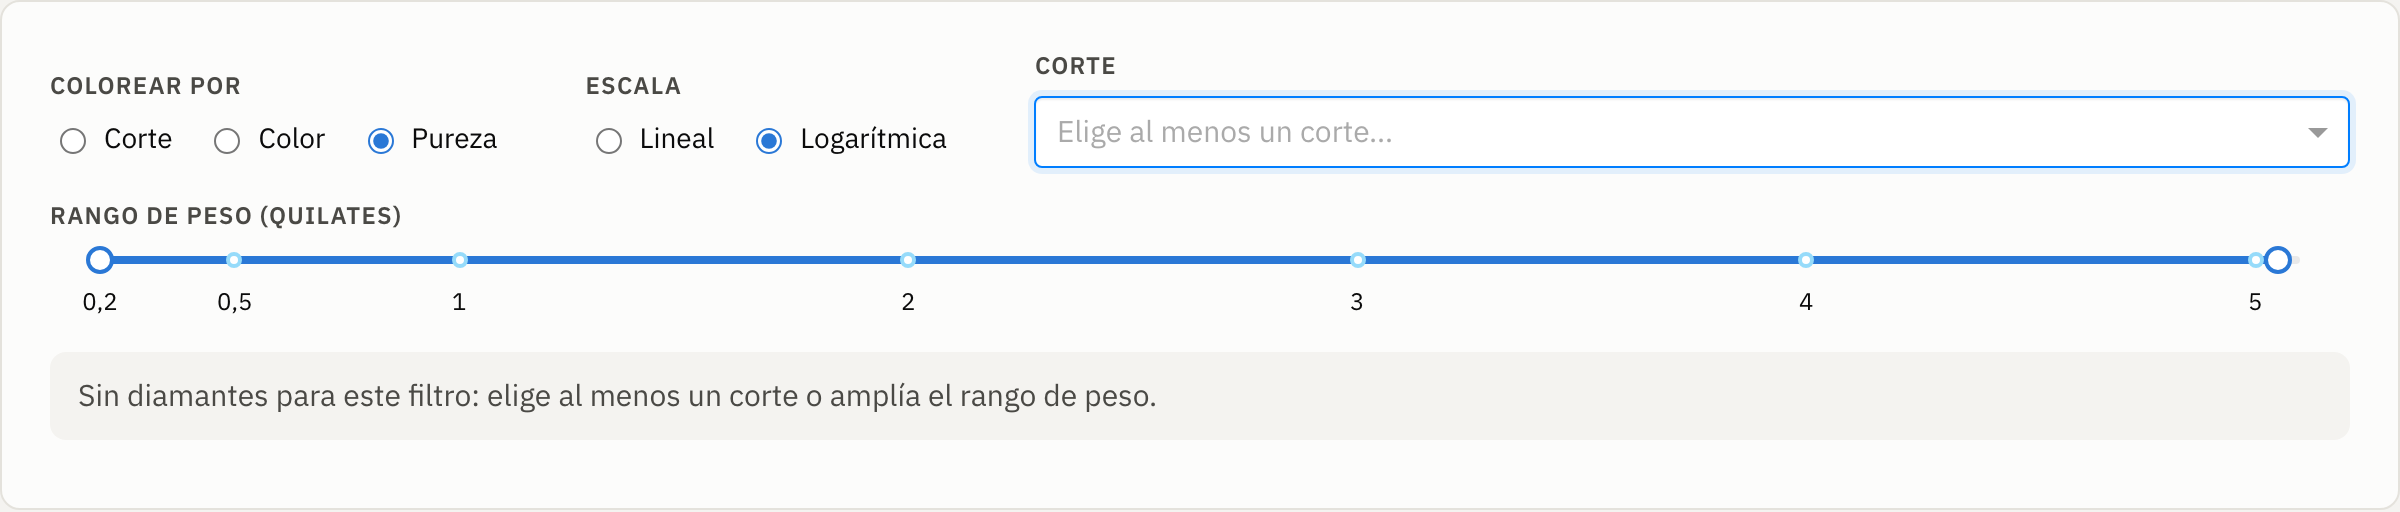
\includegraphics[width=\textwidth]{figuras/vacio-filtros}
\end{minipage}\hfill
\begin{minipage}{0.34\textwidth}\centering
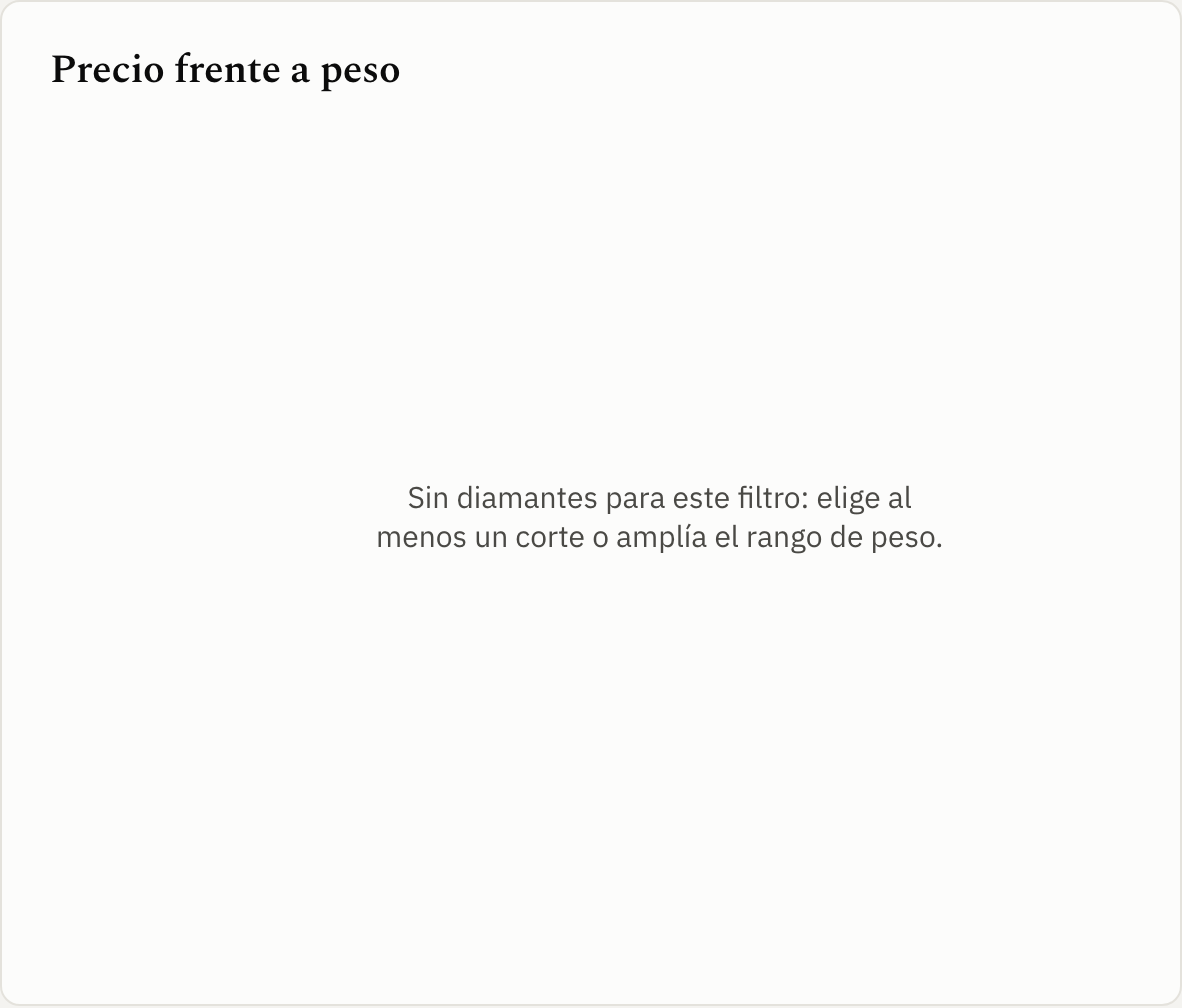
\includegraphics[width=\textwidth]{figuras/vacio-grafico}
\end{minipage}
\caption{Estado vacío en la pestaña 2: el resumen y el gráfico explican cómo recuperar datos.}
\label{fig:vacio}
\end{figure}

El dashboard también se usa en el celular (Figura~\ref{fig:movil}). Por debajo de
900 píxeles las columnas se apilan, las pestañas se desplazan en horizontal y la
tabla de oportunidades tiene su propio scroll, así que la página nunca se sale
de la pantalla.

\begin{figure}[H]
\centering
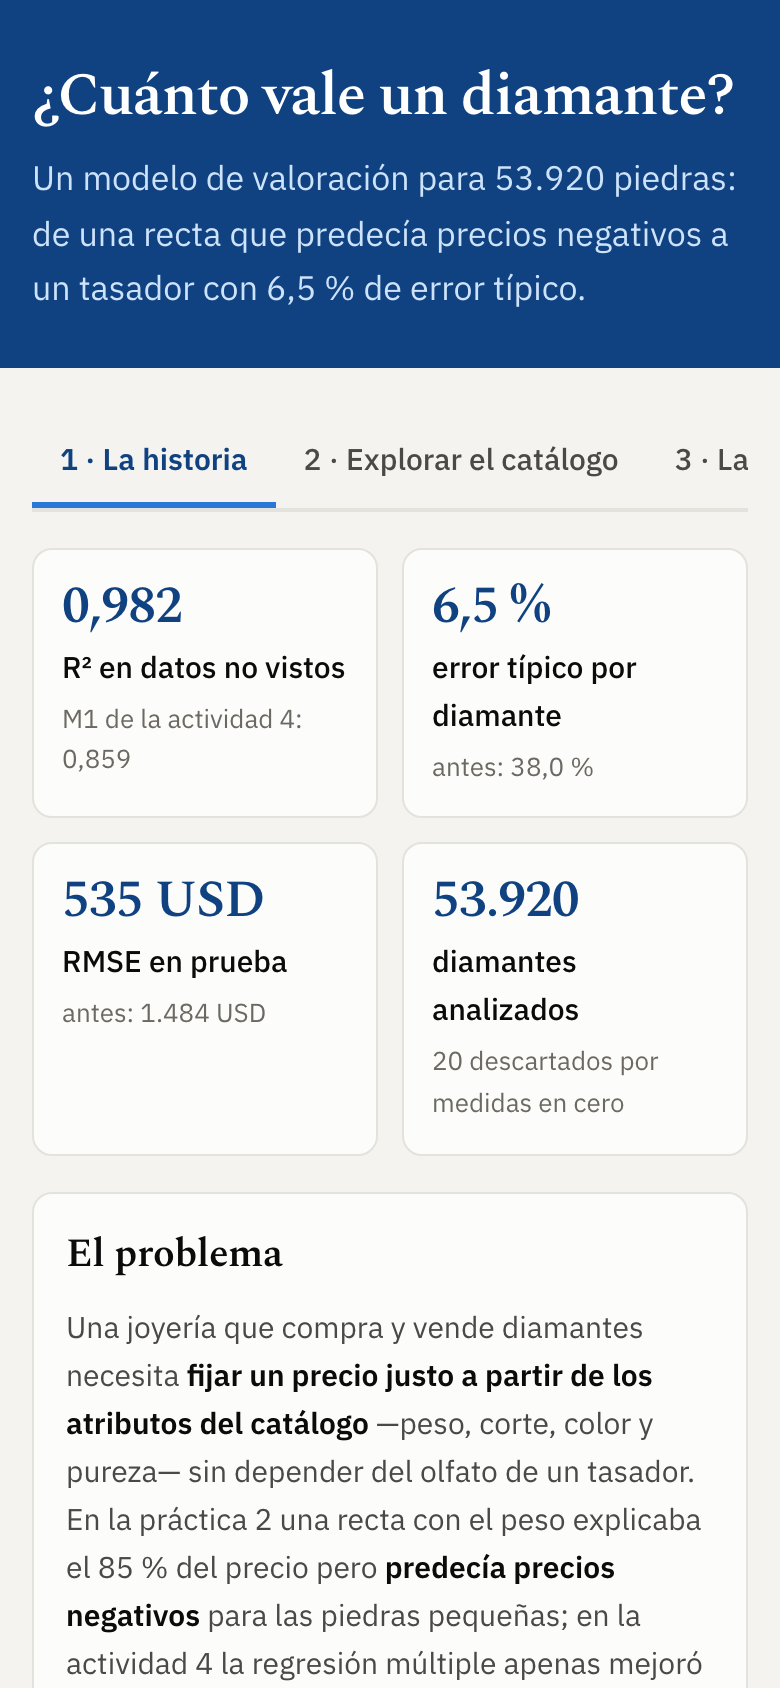
\includegraphics[width=0.31\textwidth]{figuras/movil-1}\hfill
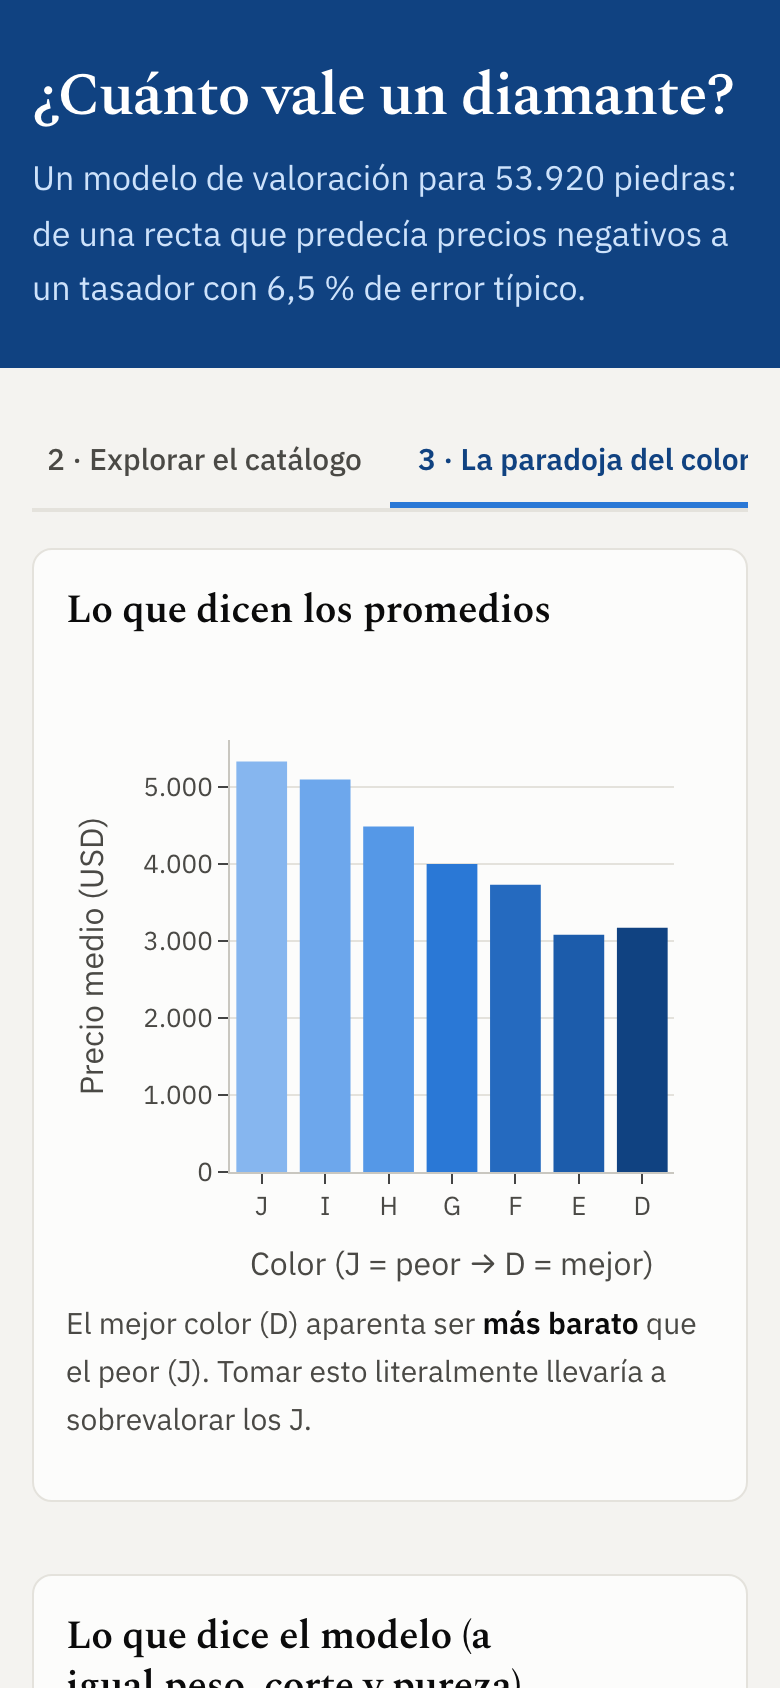
\includegraphics[width=0.31\textwidth]{figuras/movil-3}\hfill
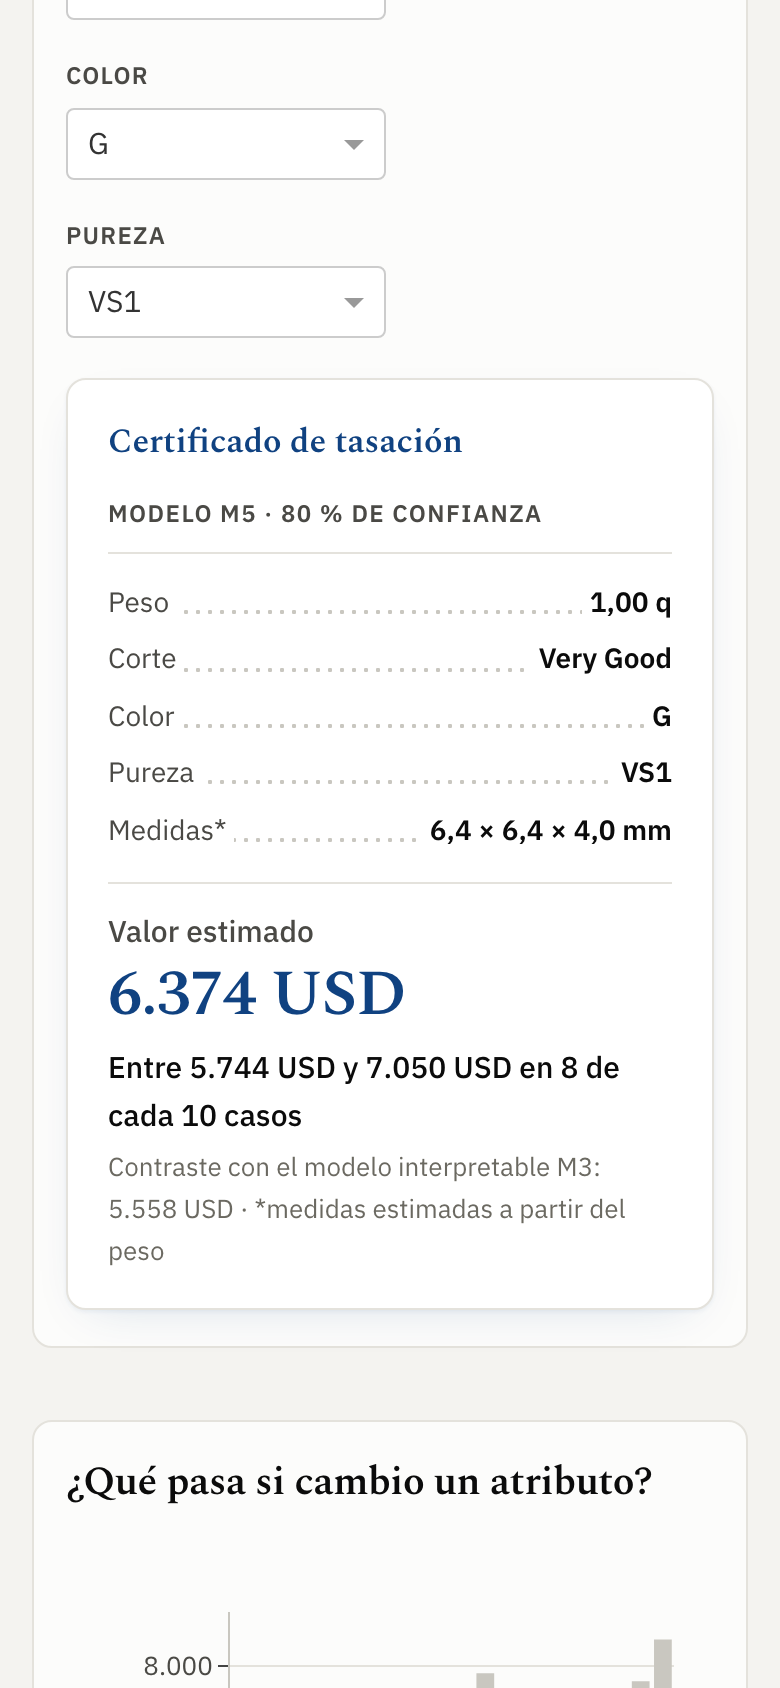
\includegraphics[width=0.31\textwidth]{figuras/movil-5}
\caption{El dashboard a 390 píxeles de ancho: la historia, la paradoja del color y el certificado de tasación.}
\label{fig:movil}
\end{figure}

\subsection{Pruebas}

\begin{itemize}[leftmargin=1.2cm,itemsep=0.25em]
\item \textbf{Prueba en navegador real.} Un script de Playwright abre el
dashboard, recorre las cinco pestañas, acciona los selectores (color, escala,
experimentos, modelo) y comprueba que no haya errores de consola ni
\emph{callbacks} fallidos. Resultado: 0 errores.
\item \textbf{Prueba en otro entorno.} Antes de publicar simulé Binder en local
(Jupyter Server con \texttt{jupyter-server-proxy} y el mismo script
\texttt{binder/start}) y repetí la prueba completa a través del proxy. Después
verifiqué el enlace real en mybinder.org, que construye la imagen desde cero en
otra máquina con las versiones fijadas en \texttt{requirements.txt}.
\item \textbf{Verificación de cifras.} El script \texttt{verificar.py} recalcula
desde el CSV crudo y los modelos guardados cada cifra citada en este informe y en
el dashboard; M0 y M1 los recalcula con NumPy puro, sin scikit-learn. Resultado:
\textbf{45 comprobaciones, 0 incorrectas}. En su primera ejecución detectó una
cifra mal transcrita (el MAPE de M2), que se corrigió.
\item \textbf{Revisión visual.} La revisión de las capturas encontró problemas que
se corrigieron: un eje truncado que exageraba diferencias mínimas (se cambió por
un gráfico de puntos), etiquetas recortadas y separadores decimales en formato
inglés.
\item \textbf{Crítica de diseño y accesibilidad.} Una revisión heurística
(heurísticas de Nielsen: 27/40 en la primera versión), un detector automático de
antipatrones visuales y una auditoría con axe-core encontraron cinco problemas
prioritarios, que se corrigieron:
\begin{itemize}[leftmargin=0.8cm,itemsep=0.1em]
\item las pestañas no se podían usar con teclado; ahora se recorren con Tab y las flechas;
\item la página no declaraba el idioma;
\item en el celular la tabla desbordaba la pantalla;
\item los filtros vacíos dejaban gráficos rotos; ahora muestran un mensaje que dice qué hacer;
\item algunos textos no alcanzaban el contraste AA.
\end{itemize}
Además, el resultado del tasador se rediseñó como un \emph{certificado de
tasación} y se agregó una guía de las escalas gemológicas (Fair→Ideal, J→D,
I1→IF) y de las métricas. Tras los cambios, axe no reporta fallos de contraste, y
los avisos que quedan pertenecen a componentes internos de Dash (desplegables,
deslizadores y paginación de la tabla).
\end{itemize}

\subsection{Manual de uso}

\begin{enumerate}[leftmargin=1.2cm,itemsep=0.2em]
\item \textbf{Sin instalar nada:} abrir el enlace de Binder del archivo
\texttt{enlaces.txt}. La primera carga puede tardar unos minutos mientras Binder
prepara el entorno; el dashboard aparece directamente.
\item \textbf{En un equipo local:} con Python 3.12,
\texttt{pip install -r requirements.txt} y luego \texttt{python app.py}. El
dashboard queda en \url{http://127.0.0.1:8050}.
\item \textbf{Para regenerar los resultados:} \texttt{python modelo.py} (unos 3
minutos) y luego \texttt{python verificar.py}.
\end{enumerate}

\section{Conclusiones}

\textbf{Sobre el modelo.} En seis iteraciones el error típico de tasación pasó
de 38,0\,\% a \textbf{6,5\,\%} ($R^2$ de 0,8587 a 0,9816), sin predicciones
negativas y con un intervalo del 80\,\% cuya cobertura se verificó en datos no
vistos. El salto decisivo fue entender que el precio es multiplicativo
(transformación log-log), no el algoritmo. La regularización se probó con rigor y
resultó innecesaria, porque el modelo lineal no sobreajustaba. El boosting ganó
porque aprende interacciones que el modelo lineal solo captura a medias.

\textbf{Sobre el problema.} El mercado paga el peso de forma más que
proporcional (elasticidad 1,88). La pureza pesa más que el color, y el color más
que el corte: pasar de I1 a IF triplica el precio (+208\,\%), mientras que el
mejor corte frente al peor solo suma un 18\,\%. El color sí se paga (D vale un
67\,\% más que J a igualdad del resto), aunque los promedios brutos digan lo
contrario. Para un comprador, el corte es donde más se ahorra; para un vendedor,
el detector de oportunidades señala precios mal fijados.

\textbf{Planteamientos para seguir.} (1) Recolectar variables nuevas
(certificado, fluorescencia, proporciones), porque la curva de aprendizaje
muestra que más filas del mismo tipo ya no mejoran el modelo. (2) Validar con
precios actuales, porque el conjunto de datos es histórico. (3) Pedir las medidas
reales en el tasador en lugar de estimarlas a partir del peso, como hace hoy la
interfaz.

\section*{Referencias}

\begin{itemize}[leftmargin=1.2cm,itemsep=0.3em]
\item Oehlert, G. W. (2010). \textit{A First Course in Design and Analysis of Experiments}. University of Minnesota.
\item Plotly. (2023, 30 de agosto). \textit{Dash Documentation}. \url{https://dash.plotly.com/}
\item The Turing Way Community. (2021). \textit{Zero to Binder}. \url{https://the-turing-way.netlify.app/communication/binder/zero-to-binder.html}
\item Kohavi, R., Longbotham, R., Sommerfield, D., \& Henne, R. M. (2008). Controlled experiments on the web: survey and practical guide. \textit{Data Mining and Knowledge Discovery, 18}(1), 140--181.
\item Hastie, T., Tibshirani, R., \& Friedman, J. (2009). \textit{The Elements of Statistical Learning} (2.ª ed.). Springer. (Regla de un error estándar, §7.10.)
\item Pedregosa, F. et al. (2011). Scikit-learn: Machine learning in Python. \textit{Journal of Machine Learning Research, 12}, 2825--2830.
\item Wickham, H. (2016). \textit{ggplot2: Elegant Graphics for Data Analysis}. Springer. (Conjunto de datos \texttt{diamonds}.)
\end{itemize}

\end{document}
